% arXiv-safe: pdfLaTeX, Computer Modern, no shell-escape.
% Every table is \input from tables/ and every in-prose number is a macro from
% numbers.tex — both GENERATED by `make paper`. Do not type a number by hand.
\documentclass[11pt]{article}

\usepackage[a4paper,margin=2.6cm]{geometry}
\usepackage{amsmath,amssymb}
\usepackage{booktabs}
\usepackage{graphicx}
\usepackage{caption}
\usepackage{microtype}
\usepackage[numbers,sort&compress]{natbib}
\usepackage[colorlinks=true,linkcolor=blue!50!black,citecolor=blue!50!black,urlcolor=blue!50!black]{hyperref}

\graphicspath{{figures/}}
\captionsetup{font=small,labelfont=bf}
\setlength{\parskip}{0.35em}

% GENERATED by paper/tables.py — do not edit by hand
\newcommand{\aFiveBocpdDelay}{17}
\newcommand{\aFiveBocpdFar}{0.13}
\newcommand{\aFiveBocpdHits}{2/16}
\newcommand{\aFiveBocpdRecall}{12\%}
\newcommand{\aFiveNOneDelay}{14}
\newcommand{\aFiveNOneFar}{2.33}
\newcommand{\aFiveNOneHits}{14/16}
\newcommand{\aFiveNOneRecall}{88\%}
\newcommand{\aFiveNTwoDelay}{12}
\newcommand{\aFiveNTwoFar}{0.19}
\newcommand{\aFiveNTwoHits}{6/16}
\newcommand{\aFiveNTwoRecall}{38\%}
\newcommand{\aFiveOutages}{16}
\newcommand{\aFiveTerminalYears}{54}
\newcommand{\aFourAlpha}{0.251}
\newcommand{\aFourClim}{2.088}
\newcommand{\aFourCov}{72.6\%}
\newcommand{\aFourMae}{2.104}
\newcommand{\aFourPersist}{2.694}
\newcommand{\aFourSkill}{+0.7\%}
\newcommand{\aFourWindow}{7.0}
\newcommand{\aOneClim}{1.814}
\newcommand{\aOneCov}{73.7\%}
\newcommand{\aOneMae}{2.314}
\newcommand{\aOnePersist}{2.217}
\newcommand{\aOneSkill}{+28\%}
\newcommand{\aTwoBallastCoef}{-0.049}
\newcommand{\aTwoClim}{2.152}
\newcommand{\aTwoMae}{3.961}
\newcommand{\aTwoSkill}{+84.0\%}
\newcommand{\bGridHiCov}{2025-12-29}
\newcommand{\bGridHiFull}{2026-08-03}
\newcommand{\bGridLoCov}{2018-01-01}
\newcommand{\bGridLoFull}{2018-01-01}
\newcommand{\bMTwoSkillHFourCov}{-18.2\%}
\newcommand{\bMTwoSkillHFourFull}{-19.2\%}
\newcommand{\bMTwoSkillHOneCov}{-9.3\%}
\newcommand{\bMTwoSkillHOneFull}{-10.4\%}
\newcommand{\bMZeroMaeHFourCov}{3.942}
\newcommand{\bMZeroMaeHFourFull}{3.947}
\newcommand{\bMZeroMaeHOneCov}{2.034}
\newcommand{\bMZeroMaeHOneFull}{1.997}
\newcommand{\bMaxRsqCov}{0.009}
\newcommand{\bMaxRsqFull}{0.009}
\newcommand{\bMaxTCov}{1.50}
\newcommand{\bMaxTFull}{1.72}
\newcommand{\bTransitTFourCov}{+1.40}
\newcommand{\bTransitTFourFull}{+1.03}
\newcommand{\bTransitTOneCov}{+0.18}
\newcommand{\bTransitTOneFull}{+0.08}
\newcommand{\bWeeksCov}{379}
\newcommand{\bWeeksFull}{395}
\newcommand{\bonferroniT}{2.394}
\newcommand{\captureTwentyEighteen}{74\%}
\newcommand{\captureTwentyFive}{105\%}
\newcommand{\captureTwentyFour}{103\%}
\newcommand{\captureTwentyThree}{93\%}
\newcommand{\captureTwentyTwenty}{46\%}
\newcommand{\coverageDropShare}{91\%}
\newcommand{\euDemandBcm}{350}
\newcommand{\fixSpanHi}{2026-08-10}
\newcommand{\fixSpanLo}{2016-01-01}
\newcommand{\gfwEnds}{2026-02-21}
\newcommand{\hOnePersistWFour}{5.25}
\newcommand{\hOneSkillWFour}{+86.7\%}
\newcommand{\hOneSkillWOne}{-27.5\%}
\newcommand{\hOneSkillWTwo}{-19.6\%}
\newcommand{\hOneTruthWFour}{0.75}
\newcommand{\hOneTruthWOne}{5.89}
\newcommand{\hacLagRule}{$h+1$}
\newcommand{\leakBounded}{4,713}
\newcommand{\leakDeclared}{2,101}
\newcommand{\leakFutureClosed}{13,130}
\newcommand{\leakFutureShare}{65\%}
\newcommand{\leakNaive}{20,351}
\newcommand{\mechDiscHiCov}{2024-12-30}
\newcommand{\mechDiscHiFull}{2024-12-30}
\newcommand{\mechDiscLoCov}{2018-01-01}
\newcommand{\mechDiscLoFull}{2018-01-01}
\newcommand{\mechDiscNCov}{327}
\newcommand{\mechDiscNFull}{327}
\newcommand{\mechHFourLooseBetaCov}{$-2.25 \times 10^{-7}$}
\newcommand{\mechHFourLooseBetaFull}{$-2.25 \times 10^{-7}$}
\newcommand{\mechHFourLooseHoldCov}{--}
\newcommand{\mechHFourLooseHoldFull}{--}
\newcommand{\mechHFourLooseTCov}{-1.00}
\newcommand{\mechHFourLooseTFull}{-1.00}
\newcommand{\mechHFourTightBetaCov}{$-1.13 \times 10^{-7}$}
\newcommand{\mechHFourTightBetaFull}{$-1.13 \times 10^{-7}$}
\newcommand{\mechHFourTightHoldCov}{$2.71 \times 10^{-7}$}
\newcommand{\mechHFourTightHoldFull}{$9.21 \times 10^{-7}$}
\newcommand{\mechHFourTightTCov}{-0.17}
\newcommand{\mechHFourTightTFull}{-0.17}
\newcommand{\mechHThreeBetaCov}{$4.78 \times 10^{-9}$}
\newcommand{\mechHThreeBetaFull}{$4.78 \times 10^{-9}$}
\newcommand{\mechHThreeHoldCov}{$-1.49 \times 10^{-9}$}
\newcommand{\mechHThreeHoldFull}{$6.73 \times 10^{-10}$}
\newcommand{\mechHThreeTCov}{+0.46}
\newcommand{\mechHThreeTFull}{+0.46}
\newcommand{\mechHTwoBetaCov}{$-2.64 \times 10^{0}$}
\newcommand{\mechHTwoBetaFull}{$-2.64 \times 10^{0}$}
\newcommand{\mechHTwoHoldCov}{$-2.51 \times 10^{0}$}
\newcommand{\mechHTwoHoldFull}{$8.23 \times 10^{0}$}
\newcommand{\mechHTwoTCov}{-0.89}
\newcommand{\mechHTwoTFull}{-0.89}
\newcommand{\mechHoldHiCov}{2025-12-01}
\newcommand{\mechHoldHiFull}{2026-07-06}
\newcommand{\mechHoldLoCov}{2025-01-06}
\newcommand{\mechHoldLoFull}{2025-01-06}
\newcommand{\mechHoldNCov}{48}
\newcommand{\mechHoldNFull}{64}
\newcommand{\mechLooseCov}{162}
\newcommand{\mechLooseFull}{162}
\newcommand{\mechMaxTCov}{0.89}
\newcommand{\mechMaxTFull}{0.89}
\newcommand{\mechTightCov}{213}
\newcommand{\mechTightFull}{229}
\newcommand{\mechTrendRsqCov}{0.209}
\newcommand{\mechTrendRsqFull}{0.209}
\newcommand{\nBackfillEvents}{84,636}
\newcommand{\nEvents}{87,874}
\newcommand{\nFixes}{54,494,686}
\newcommand{\nFleet}{828}
\newcommand{\nLadenDepartures}{9,855}
\newcommand{\nLiveEvents}{3,238}
\newcommand{\nPanelFeatures}{20}
\newcommand{\nPanelRows}{77,500}
\newcommand{\nSignalKeys}{34}
\newcommand{\nSignalRows}{1,032,982}
\newcommand{\noaaEnds}{2025-12-31}
\newcommand{\powerFloor}{1.72\%}
\newcommand{\powerN}{327}
\newcommand{\seasonalityRatio}{1.35}
\newcommand{\spreadWeeklySd}{11.22}
\newcommand{\stockDaysDemand}{2.3}
\newcommand{\stockDecTwentyFive}{4.80}
\newcommand{\stockJanTwentySix}{0.41}
\newcommand{\stockMeanBcm}{2.21}
\newcommand{\stockMeanMm}{3.69}
\newcommand{\stockSdDaysDemand}{1.37}
\newcommand{\vintagePostDay}{68}
\newcommand{\vintageSameDay}{909}


\newcommand{\spread}{\ensuremath{s_t}}
\newcommand{\HH}{Henry Hub}
\newcommand{\TTF}{TTF}
\newcommand{\Rsq}{\ensuremath{R^2}}
\newcommand{\pRsq}{partial \ensuremath{R^2}}

\title{Public vessel-tracking data does not predict the Henry Hub--TTF spread:\\
  a pre-registered, power-bounded null}
\author{Alec Mitchell-Thomson\\\small Independent researcher}
\date{\today\quad\small (first draft)}

\begin{document}
\maketitle

\begin{abstract}
Positions of liquefied-natural-gas carriers are widely believed to carry
information about the price gap between North American and European gas: a cargo
that leaves the US Gulf today lands in Europe in two to three weeks, and that
supply is not yet in any published statistic. We test the belief directly. From
\nFixes{} AIS position fixes (\fixSpanLo{} to \fixSpanHi{}), reconstructed into
\nEvents{} port events and a \nSignalKeys-signal daily panel built twice --- once
with hindsight for validation and once strictly point-in-time for modelling --- we
ask whether tanker-derived signals predict the one- and four-week change in the
\HH{}--\TTF{} spread net of its own persistence, weather, storage and oil. Every
hypothesis, sign and acceptance bar was committed to a dated append-only log before
the corresponding fit. The answer is no. A controls-only model is worse than
assuming no change (\bMTwoSkillHOneCov{} at one week, \bMTwoSkillHFourCov{} at four);
no signal reaches a Newey--West $|t|$ of 1.96 (maximum \bMaxTCov); and three
pre-registered mechanisms that could hide an effect from a linear scan --- the
Europe-bound \emph{share} of cargo, an interaction with EU storage, and a
tightness-regime split --- fail under a Bonferroni bar with an untouched holdout.
The design detects effects of at least \powerFloor{} of residual variance and
observed at most \bMaxRsqCov, so the result rules out tradeable effects and is
silent on sub-tradeable ones. Alongside the null, we document two construction
hazards specific to voyage-derived features: the unit of observation is defined
retrospectively, and feature \emph{availability} changes across data vintages. A
naive loader leaked \leakFutureShare{} of the sample.
\end{abstract}

% PROPOSAL: the author rewrites this section. It states the claim as the
% generated numbers support it. Framing and emphasis are the author's decision.
\section{Introduction}

The Henry Hub--TTF spread is the price of moving a unit of gas from the United
States to Europe, and liquefied natural gas (LNG) carriers are the means by which it
moves. A laden carrier that leaves Sabine Pass arrives at Rotterdam roughly fourteen
to eighteen days later. Between departure and arrival its cargo is committed, is
visible to anyone with an AIS receiver, and is absent from every published supply
statistic. It is therefore natural to expect vessel positions to lead the spread.
This expectation is widely held and is the basis of a commercial data industry.

This paper tests it and finds no support. An efficient-markets view predicts that
outcome, so the null itself is not the contribution. The contribution lies in how
the null is established, and in two construction problems encountered on the way.

Three features of the design distinguish the result from a mere absence of findings.
First, every target, control set, lag, sign and acceptance bar was written into a
dated, append-only decision log before the corresponding fit, so no choice reported
below was made after seeing its outcome. Where a pre-registered sign was falsified,
it is reported as falsified. Second, the inference respects the structure of the
data. Weekly changes over a four-week horizon overlap, so all standard errors are
Newey--West with the lag fixed in advance at \hacLagRule{} weeks. Training rows whose
target reaches into the test week are purged. The three follow-up mechanism tests
are held to a Bonferroni bar and must replicate their sign on a holdout that was not
examined until they had passed on the discovery sample. Third, the study bounds
what it could have found. With \powerN{} weekly observations the design detects
effects of at least \powerFloor{} of residual variance, and the largest observed
anywhere is \bMaxRsqCov. The result excludes effects large enough to trade and is
silent on smaller ones.

Two further findings are methodological and apply to any feature built from
vessel-tracking data. The natural unit of observation, a voyage, does not exist
until both of its endpoints have been observed, so a statistic computed over
completed voyages embeds the future unless the population is explicitly bounded. At
a 2020 as-of date a straightforward loader returned \leakNaive{} legs, of which
\leakFutureClosed{} (\leakFutureShare) had been closed by arrivals that had not yet
occurred. Separately, the availability of a feature can change across data vintages.
The same loader attached \leakDeclared{} destination declarations to 2020 voyages
from a data feed that began in 2026. A date filter on observations cannot catch
this, because the individual rows are correctly dated; the table itself should not
exist at that vintage.

The paper proceeds as follows. Section~\ref{sec:data} describes the pipeline and
the decade-scale reconstruction. Section~\ref{sec:panel} explains how the signal
panel is built point-in-time. Section~\ref{sec:prereg} describes the
pre-registration protocol and its limits. Section~\ref{sec:parta} reports the
physical nowcasts. Section~\ref{sec:partb} reports the spread tests.
Section~\ref{sec:power} bounds their power. Sections~\ref{sec:discussion}
and~\ref{sec:limitations} interpret and qualify the results.

\section{Data and pipeline}\label{sec:data}

\begin{figure*}[tb]
\centering
\resizebox{\textwidth}{!}{% The pipeline, sources to paper. Hand-laid-out (a diagram, not a measurement);
% every count on it is a macro from numbers.tex / numbers2.tex.
\begin{tikzpicture}[
  x=1cm, y=1cm,
  box/.style={draw=ink, rounded corners=1.5pt, fill=white, inner sep=2.5pt,
              align=center, font=\scriptsize, minimum height=7mm, text width=2.55cm},
  src/.style={box, fill=paleblue},
  store/.style={box, fill=palegold},
  derive/.style={box, fill=palegrey},
  outbox/.style={box, fill=white, draw=ink, thick},
  arr/.style={-{Latex[length=1.5mm]}, draw=ink!75, line width=0.5pt},
  lab/.style={font=\tiny, fill=white, inner sep=1pt, text=ink!80},
]
% ---- row 1: sources
\node[src] (igu)  at (1.5, 4.3) {IGU fleet list\\ \tiny annual PDF};
\node[src] (ais)  at (4.7, 4.3) {AISstream\\ \tiny 3 WebSockets per worker, 150 MMSI slots, 1\,h rotation};
\node[src] (vf)   at (7.9, 4.3) {VesselFinder API\\ \tiny masterdata; credit-budgeted rescue};
\node[src] (noaa) at (11.1, 4.3) {NOAA Marine Cadastre\\ \tiny US Class-A AIS, 2016--25};
\node[src] (gfw)  at (14.3, 4.3) {Global Fishing Watch\\ \tiny port visits and voyages, 2016--26};
% ---- row 2: stores
\node[store] (reg) at (1.5, 2.7) {\texttt{vessel\_registry}\\ \tiny \nFleet{} LNG carriers and FSRUs};
\node[store] (fix) at (6.3, 2.7) {\texttt{ais\_fixes}\\ \tiny \nFixes{} fixes (hypertable)};
\node[derive] (sm) at (9.5, 2.7) {state machine\\ \tiny per vessel, \nZonePolygons{} polygons at \nTerminals{} terminals};
\node[store] (pe) at (12.7, 2.7) {\texttt{port\_events}\\ \tiny \nEvents{} events, regime-tagged};
\node[src] (mkt) at (15.9, 2.7) {EIA, FRED, AGSI+,\\ ERA5, TTF quote\\ \tiny prices, storage, weather};
% ---- row 3: derivations
\node[derive] (wl) at (3.9, 1.1) {\texttt{priority\_watchlist}\\ \tiny 5 tiers, re-scored hourly};
\node[derive] (pair) at (9.5, 1.1) {legs, visits, queues\\ \tiny the three pairings};
\node[store] (sd) at (12.7, 1.1) {\texttt{signal\_daily}\\ \tiny \nSignalKeys{} keys, two bases, \nSignalRows{} rows};
\node[store] (mp) at (15.9, 1.1) {\texttt{model\_panel}\\ \tiny \nPanelFeatures{} features, publication-lagged};
% ---- row 4: analysis and paper
\node[outbox] (parta) at (9.5, -0.5) {Part A replays\\ \tiny A1, A2, A4, A5 nowcasts};
\node[outbox] (partb) at (12.7, -0.5) {Part B replays\\ \tiny M0--M2 ladder, FWL scan, H2--H4};
\node[outbox] (paper) at (15.9, -0.5) {tables, macros, figures\\ \tiny generated, never typed};
% ---- edges
\draw[arr] (igu) -- (reg);
\draw[arr] (vf) -- node[lab, pos=0.62] {IMO$\to$MMSI} (reg);
\draw[arr] (ais) -- (fix);
\draw[arr] (vf) -- node[lab, pos=0.55] {rescue fixes} (fix);
\draw[arr] (noaa) -- node[lab, pos=0.5] {backfill} (fix);
\draw[arr] (fix) -- (sm);
\draw[arr] (sm) -- (pe);
\draw[arr] (gfw) -- node[lab, pos=0.5] {events written directly} (pe);
\draw[arr] (reg.south) |- (wl.west);
\draw[arr] (fix.south west) -- node[lab, pos=0.5, right=1pt] {last fix, ETA, destination} (wl.north east);
\draw[arr] (wl.north) -- node[lab, pos=0.22, left=1pt] {subscription list} (ais.south);
\draw[arr] (pe) -- (pair);
\draw[arr] (pair) -- (sd);
\draw[arr] (sd) -- (mp);
\draw[arr] (mkt) -- (mp);
\draw[arr] (pair) -- (parta);
\draw[arr] (mp) -- (partb);
\draw[arr] (parta) -- (partb);
\draw[arr] (partb) -- (paper);
\end{tikzpicture}
}
\caption{The pipeline from sources to paper. Blue boxes are external sources, gold
boxes are stored tables, grey boxes are derivations, and the outlined boxes are the
replays that generate every table and figure. The watchlist closes a loop: the
ranking computed from stored fixes decides which vessels the live feed subscribes
to next.}
\label{fig:pipeline}
\end{figure*}

\subsection{Sources}

Vessel positions come from three feeds of different fidelity, and no signal is
aggregated across the boundary between them. For the United States we use the NOAA
Marine Cadastre archive of terrestrial Class-A AIS \citep{noaa_ais}, which is
exhaustive along the US coast from 2016 and ends on \noaaEnds. For Europe and the
open ocean we use Global Fishing Watch port-visit and voyage events \citep{gfw}.
These supply arrivals and departures but carry no coordinates and no anchorage
events; the feed ends on \gfwEnds. A live subscription to an AIS aggregator covered a
tier-ranked fleet from April~2026 (Section~\ref{sec:live}) and is used only for the
vintage self-validation described in Section~\ref{sec:panel}.

The fleet in scope is every LNG carrier and floating storage and regasification
unit (FSRU) in the IGU fleet list, \nFleet{} hulls, resolved to an MMSI through a
vessel-database lookup. The signals concern the transatlantic subset of their
movements: laden departures from US export terminals, arrivals and discharges at
European import terminals, and the ballast return. Cargoes bound for Asia or Latin
America enter the panel only as an unresolved-destination band
(Section~\ref{sec:partb}).

Prices and controls are public. \HH{} spot and Lower-48 storage are from the EIA API
\citep{eia_api}. The TTF front-month contract is from a keyless quote feed and was
cross-checked against the World Bank's monthly European gas series
\citep{worldbank_cmo}; the regression slope is 0.999 with $\Rsq=0.9999$ over 106
months, so the distortion introduced by the continuous roll is negligible. EUR/USD
and Brent are from FRED \citep{fred}. EU storage is from GIE AGSI+ \citep{agsi}.
Heating and cooling degree days are computed from ERA5 reanalysis temperatures at
weighted demand centres \citep{openmeteo}.

\subsection{Reconstruction}\label{sec:reconstruction}

Table~\ref{tab:inventory} gives the scale of the reconstruction and
Figure~\ref{fig:pipeline} its shape. Fixes are resolved against \nZonePolygons{}
polygons at \nTerminals{} terminals in seven zones (US Gulf, US Atlantic, north-west
Europe, Baltic, Iberia, western Mediterranean and eastern Mediterranean). The
polygons were drawn by hand in QGIS from satellite imagery and port charts, one
berth, one anchorage and one approach envelope per terminal, with sub-zones where a
terminal has several berths. The approach envelope is deliberately drawn to contain
the anchorage, the channel and the berth, so that a single visit stays open while a
vessel transits between them; without it the four-to-six hour channel transit at
Sabine Pass or Rotterdam would register as a departure and a fresh arrival.
Figure~\ref{fig:zones} shows the three polygons at Sabine Pass with a sample of the
events emitted inside them.

\begin{table*}[tb]
\centering\small
\caption{Reconstruction inventory. Port events are labelled by the feed that produced
them. The two backfill feeds end months before the live feed, which determines the
sample choice in Section~\ref{sec:partb}.}
\label{tab:inventory}
\begin{tabular}{lrl}
\toprule
layer & rows & span \\
\midrule
AIS position fixes & 54,494,686 & 2016-01-01 to 2026-08-10 \\
port events (state machine) & 87,874 & \\
  \quad noaa & 44,363 & to 2025-12-31 \\
  \quad gfw & 40,273 & to 2026-02-21 \\
  \quad mmsi\_filter & 1,974 & to 2026-08-10 \\
  \quad bbox & 1,264 & to 2026-05-30 \\
in-scope fleet (LNG carriers + FSRUs) & 828 & \\
laden US export departures & 9,855 & \\
signal panel rows (\texttt{signal\_daily}) & 1,032,982 & 34 keys, two bases \\
model panel rows (\texttt{model\_panel}) & 77,500 & 20 features \\
\bottomrule
\end{tabular}

\end{table*}

\begin{figure}[t]
\centering
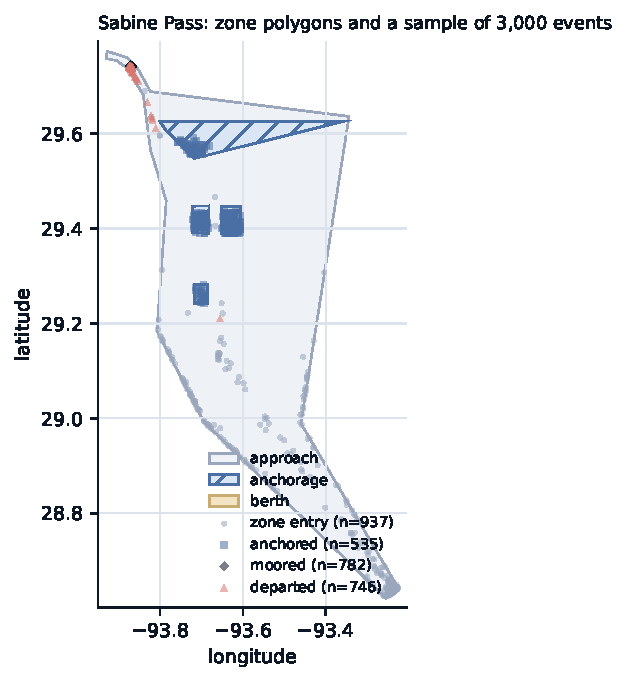
\includegraphics[width=\linewidth]{fig7_zones}
\caption{The hand-drawn polygons at \zoneFigureTerminal{} and a random sample of
the \nZoneFigureEvents{} coordinate-bearing events the state machine emitted there.
The approach envelope (light) contains the anchorage (hatched) and the berth (gold,
at the head of the channel). Zone entries scatter along the envelope boundary,
anchored events cluster in the anchorage boxes, and moored and departed events sit
on the berth.}
\label{fig:zones}
\end{figure}

\begin{figure*}[tb]
\centering
\resizebox{0.78\textwidth}{!}{% The per-vessel state machine (pipeline/state_machine.py). Thresholds are the
% code's defaults: 30 min dwell at SOG < 1 kn for anchored/moored, 15 min at
% SOG > 1 kn outside the berth for departed. Events fire back-dated to the first
% qualifying fix, not to the fix that confirmed the dwell.
\begin{tikzpicture}[
  x=1cm, y=1cm,
  st/.style={draw=ink, rounded corners=2pt, fill=palegrey, font=\scriptsize\bfseries,
             inner sep=3pt, minimum width=1.9cm, minimum height=6mm},
  ev/.style={font=\tiny, align=center, fill=white, inner sep=1pt},
  arr/.style={-{Latex[length=1.5mm]}, draw=ink, line width=0.55pt},
]
\node[st] (T) at (0, 0) {TRANSIT};
\node[st] (E) at (4.2, 0) {IN\_ENVELOPE};
\node[st] (A) at (8.8, 1.9) {ANCHORED};
\node[st] (M) at (8.8, -1.9) {MOORED};
\node[st] (D) at (13.2, -1.9) {DEPARTED};
\draw[arr] (T) -- node[ev, below, yshift=-2pt] {\texttt{zone\_entry}\\first fix inside\\the approach envelope} (E);
\draw[arr] (E) -- node[ev, below right, pos=0.55, xshift=-2pt, yshift=-1pt] {\texttt{anchored}\\$\ge$30\,min at SOG$<$1\,kn\\in the anchorage} (A);
\draw[arr] (E) -- node[ev, below left, pos=0.5, xshift=2pt, yshift=-1pt] {\texttt{moored}\\$\ge$30\,min at SOG$<$1\,kn\\in a berth} (M);
\draw[arr] (A) -- node[ev, right] {\texttt{moored}} (M);
\draw[arr] (A) to[bend right=38] node[ev, above, yshift=3pt] {\texttt{anchorage\_exit}} (E);
\draw[arr] (M) -- node[ev, above, yshift=2pt] {\texttt{departed}\\SOG$>$1\,kn outside\\the berth for 15\,min} (D);
\draw[arr] (D) to[bend left=30] node[ev, below, yshift=-3pt] {\texttt{zone\_exit}: first fix outside the envelope} (T);
\node[ev, text=ink!70] at (4.2, 3.0) {\texttt{anchorage\_entry} / \texttt{anchorage\_exit}: raw polygon crossings, no dwell filter};
\end{tikzpicture}
}
\caption{The per-vessel state machine. Each fix is first resolved to a polygon
(berth wins over anchorage, which wins over approach; an open visit is sticky to its
terminal), then the state is advanced. Dwell-confirmed events are back-dated to the
first qualifying fix. Transitions require a fix outside the relevant polygon, so a
gap in coverage never emits an event on its own.}
\label{fig:statemachine}
\end{figure*}

A per-vessel state machine (Figure~\ref{fig:statemachine}) walks each vessel's
fixes in time order and emits zone entry, anchorage, mooring and departure events.
A vessel is \term{anchored} after at least 30 minutes inside an anchorage polygon at
speed over ground below 1\,kn, \term{moored} after the same dwell inside a berth
polygon, and \term{departed} after 15 minutes outside the berth at more than 1\,kn.
Anchorage entries and exits are raw polygon crossings with no dwell filter, so
that queue times can be measured without the half-hour back-dating of the
dwell-confirmed marker. A vessel whose first observed fix is already inside a
polygon receives synthetic entry and mooring events flagged as a cold start.

Laden state is inferred from the draught the vessel broadcasts relative to its
design draught,
\begin{equation}
  \text{laden}_e = \mathbf{1}\!\left[\, d(t_e) \ge 0.85\, d_{\mathrm{design}} \,\right],
  \label{eq:laden}
\end{equation}
where $d(t_e)$ is the most recent reported draught at or before the event time
for inbound events and, for departures, the first draught reported in a window
from one hour before to six hours after the event, because a master typically
rebroadcasts the lighter draught only after undocking. When no usable draught
exists the state is set from the terminal's flow direction: a vessel that moored at
an export terminal leaves laden, and one that moored at an import terminal leaves
in ballast.

Three pairings of those events underlie everything that follows and are drawn in
Section~\ref{sec:panel}. A \term{leg} pairs a departure with the vessel's next zone
entry and represents a voyage. A \term{visit} pairs a mooring with the next departure
and represents berth occupancy. A \term{queue} pairs the first anchorage entry with
the next mooring at the same terminal and represents the wait to berth.

\subsection{Live acquisition}\label{sec:live}

The live feed is the part of the project that took most of the engineering, and its
limits are part of the result, so it is described here even though the decade
panel is what the tests run on. The AIS aggregator caps a subscription at 50 vessel
identifiers per connection. The system therefore runs two ingester workers on
separate egress addresses, each holding three WebSocket connections: two connections
form a persistent block of 100 slots and the third is a scan rotation of 50 slots
that is re-drawn every hour, for 300 slots in total against a fleet of \nFleet.

Which vessels hold a slot is decided by a ranking recomputed hourly from stored
fixes and static data (Figure~\ref{fig:watchlist}). Tier~1 is any vessel seen
inside a terminal polygon in the last three days. Tier~2 is a vessel with a parsed
ETA within 48 hours or a declared destination that resolves to a known terminal.
Tier~3 is a vessel inside the wider zone bounding box, ordered by whether it is
closing on a terminal. Tiers~4 and~5 are recently and not recently seen. Two
classes are pinned into the persistent block regardless of tier: a vessel on an
open leg inside its expected arrival window in either direction, and a vessel
currently in port, so that a long berth queue does not decay out of coverage.
FSRUs are demoted to the lowest tier because a deployed FSRU sits moored for
months and its own fixes never drive a signal. At the time of writing
\nWatchlistSlotted{} of \nWatchlistVessels{} ranked vessels hold a slot:
\nSlotsPinned{} pinned, \nSlotsPersistent{} persistent and \nSlotsScan{} in
rotation.

\begin{figure}[t]
\centering
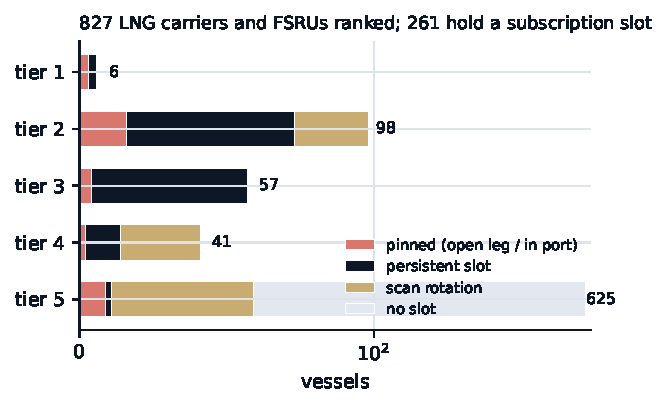
\includegraphics[width=\linewidth]{fig9_watchlist}
\caption{Subscription slots by tier at the time of writing. The horizontal axis is
symmetric-log so that the \nSlotsNone{} unslotted vessels in tier~5 do not hide the
allocation in tiers~1 to~4.}
\label{fig:watchlist}
\end{figure}

Terrestrial AIS does not see the open ocean, and a vessel that leaves a slot goes
dark until it is re-ranked. Two backstops exist. First, a vessel that goes silent
near a terminal while a leg-defining event is at risk (a laden departure, an import
arrival, a berthing) is looked up on a commercial vessel-position API and the
returned position is injected as an ordinary fix, so the state machine
re-acquires it for free. The lookups cost credits from a reserve that expires on a
fixed date, so the daily budget is derived each run as the straight line from the
current balance to zero at expiry; leg-defining classes are exempt from the line and
lower classes spend only the surplus above it (Figure~\ref{fig:rescue}). Between
the first snapshot and \vfCreditsAsOf{} the reserve fell from \vfCreditsStart{} to
\vfCreditsNow{} credits against an expiry of \vfExpiry, over \nRescueLookups{}
lookups of which \nRescued{} returned a usable position; \nRescueSkipped{} candidate
lookups were declined by the budget, which is the measured unmet demand. Second, a
daily discovery pass resolves newly delivered hulls from the fleet list, because
under a closed subscription list no vessel can otherwise enter the system.

\begin{figure*}[tb]
\centering
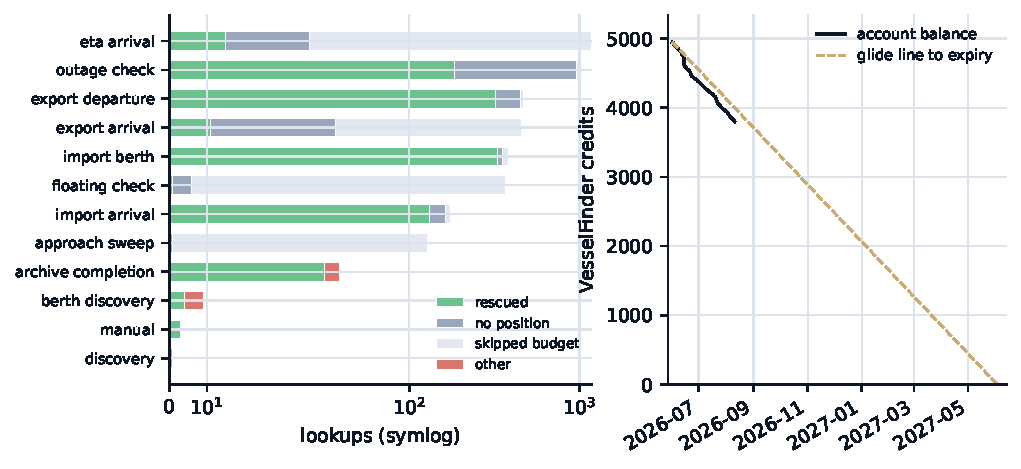
\includegraphics[width=\textwidth]{fig10_rescue}
\caption{The credit-budgeted position backstop. Left: outcomes of every lookup
attempt by rescue class, on a symmetric-log axis; green is a usable position, grey
is a lookup that returned nothing, and light grey is a candidate the budget declined.
Right: the account balance against the glide line from the first snapshot to zero at
expiry, which is the policy the daily cap is derived from.}
\label{fig:rescue}
\end{figure*}

Two limits follow directly. A vessel that was never ranked highly enough to hold
a slot leaves no live trace at all, and a vessel that drops out of coverage mid-voyage
is only recovered if it re-enters a slot or is bought back. Both are absent from the
decade archives, which is why the tests of Sections~\ref{sec:parta} and~\ref{sec:partb}
run on the NOAA and GFW backfills and the live feed serves only to validate the
point-in-time construction.

\subsection{Ground truth}\label{sec:groundtruth}

The US side of the reconstruction can be checked against a published total. The EIA
reports monthly US LNG exports $X_m$ in MMcf of gas. Dividing by a nominal cargo of
$V_c = 174{,}000$\,m$^3$ of LNG, which at a volumetric expansion of 600 is about
3.69\,Bcf of gas, gives an implied cargo count, and the ratio of observed laden
departures $D_y$ to that count is the capture rate for year $y$:
\begin{equation}
  c_y \;=\; \frac{D_y}{\sum_{m\in y} X_m \,/\, (600\,V_c)} .
  \label{eq:capture}
\end{equation}
Restricted to the NOAA feed, $c_y$ is \captureTwentyTwenty{} in 2020 and rises to
\captureTwentyThree{}, \captureTwentyFour{} and \captureTwentyFive{} in 2023, 2024
and 2025 (Table~\ref{tab:capture}, Figure~\ref{fig:capture}). The gradient is a
property of the archive, not of the vessels: the NOAA archive is assembled from
terrestrial receivers whose density along the Gulf coast grew over the decade, and
a cargo that loaded in 2020 out of range of a receiver left no fix. The GFW feed has
the opposite gradient, strong in the years the NOAA archive is thin and fading after
2022, because it is fed by satellite receptions whose coverage of the fleet
declined. The two feeds are not fused in this paper. The project's diagnostic tool
counts every feed and therefore double-counts departures seen by both, and a deduped
union calibrated to the EIA total is listed as future work
(Section~\ref{sec:future}).

\begin{table}[t]
\centering\small
\caption{NOAA-only capture of US LNG export cargoes relative to the EIA-implied count,
Equation~\eqref{eq:capture}.}
\label{tab:capture}
\begin{tabular}{lrrr}
\toprule
year & captured & EIA-implied & capture \\
\midrule
  2016 & 48 & 51 & 95\% \\
  2017 & 159 & 192 & 83\% \\
  2018 & 216 & 294 & 74\% \\
  2019 & 290 & 494 & 59\% \\
  2020 & 300 & 648 & 46\% \\
  2021 & 715 & 966 & 74\% \\
  2022 & 918 & 1048 & 88\% \\
  2023 & 1,099 & 1178 & 93\% \\
  2024 & 1,216 & 1185 & 103\% \\
  2025 & 1,570 & 1494 & 105\% \\
\bottomrule
\end{tabular}

\end{table}

\begin{figure}[t]
\centering
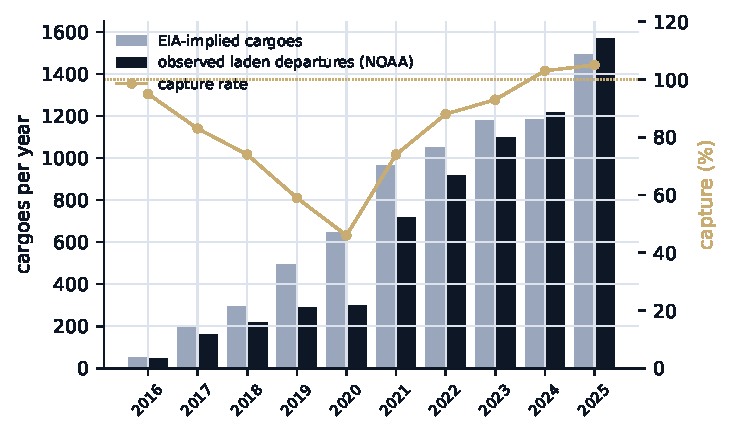
\includegraphics[width=\linewidth]{fig19_capture}
\caption{Observed laden departures against the EIA-implied cargo count by year. The
capture rate (gold, right axis) is the coverage of the NOAA archive, which is why
early-year levels of every US signal are biased low.}
\label{fig:capture}
\end{figure}

The consequence for modelling is stated here because it matters everywhere below.
Early-year levels of any US signal are biased low by up to half. The models
therefore never treat an early-year level as a physical quantity. The physical
nowcasts (Section~\ref{sec:parta}) forecast within-window changes and score against
nulls computed from the same observed series, so a uniform under-count deflates the
model and the null identically. The spread scan (Section~\ref{sec:partb})
residualises each signal on the controls and on its own past before it is used, so a
slowly varying level bias is absorbed by the persistence term. What neither design
can absorb is a level-dependent non-linearity in the early years, and that is listed
as a limitation.

Figure~\ref{fig:spread} shows the target and the headline signal on one timeline.
The two structural events that any model must survive are visible: the 2020 and
2021 inversions, in which \HH{} briefly exceeded \TTF{}, and the 2022 European
crisis.

\begin{figure*}[tb]
\centering
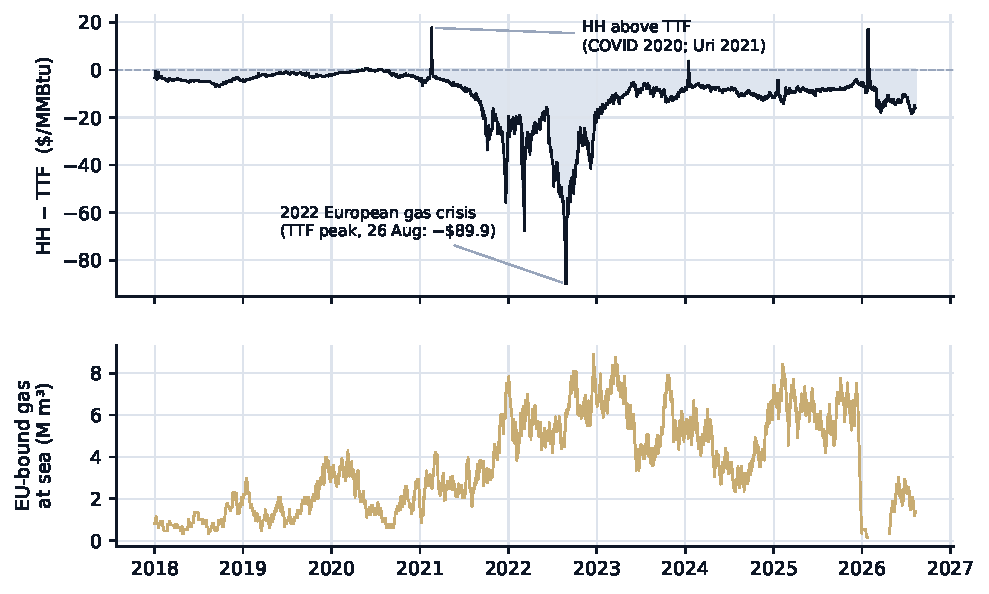
\includegraphics[width=0.92\textwidth]{fig1_spread_and_stock}
\caption{The \HH{}--\TTF{} spread (top) and EU-bound gas at sea (bottom), daily, on
the coverage-consistent sample used for modelling. The extremes coincide with Winter
Storm Uri (February~2021) and the August~2022 TTF peak. The collapse of the at-sea
stock in the final weeks is not a physical event: it is the point at which the two
backfill feeds end and only the thin live feed remains (Section~\ref{sec:seam}),
which is why the primary sample is truncated there.}
\label{fig:spread}
\end{figure*}

\section{Building the panel point-in-time}\label{sec:panel}

\begin{figure*}[tb]
\centering
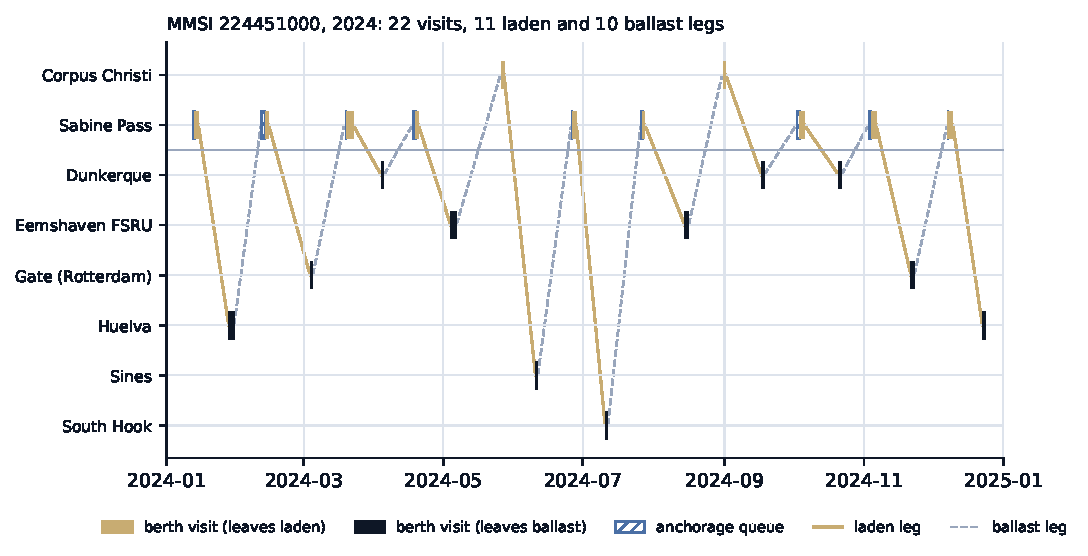
\includegraphics[width=\textwidth]{fig8_vessel_year}
\caption{One carrier's \vesselFigureYear{} as the three pairings. Each row is a
terminal, US export terminals above the rule and European import terminals below.
A gold bar is a berth visit that ends with a laden departure, a black bar one that
ends in ballast, and a hatched bar the anchorage wait before berthing. Solid lines
are laden legs from a US departure to the next European zone entry; dashed lines are
the ballast return. This vessel made \vesselFigureVisits{} visits,
\vesselFigureLadenLegs{} laden and \vesselFigureBallastLegs{} ballast legs, from
\vesselFigureEvents{} events; the US events are from the NOAA archive and the
European ones from GFW, which is why the European visits carry no anchorage wait.}
\label{fig:vessel}
\end{figure*}

Figure~\ref{fig:vessel} shows the three pairings on one vessel's year. Every
signal is built from them twice. A \term{physical} basis uses hindsight and serves
validation. A \term{knowable} basis uses, on each day $d$, only what could have been
observed on day $d$, and serves modelling.

The headline signals are gas volumes. Let leg $i$ carry capacity $V_i$ (m$^3$ of
LNG), depart at $t^{\mathrm{dep}}_i$ and arrive at $t^{\mathrm{arr}}_i$. The
physical at-sea stock on day $d$ is
\begin{equation}
  S^{\mathrm{phys}}_d = \sum_i V_i \,
    \mathbf{1}\!\left[t^{\mathrm{dep}}_i \le d < t^{\mathrm{arr}}_i\right],
  \label{eq:stock-phys}
\end{equation}
banded by the arrival zone. The knowable stock replaces the arrival test with
what is known on $d$: a leg is at sea if it has departed and no arrival has been
\emph{observed} by $d$, and it is banded by destination only if a destination was
declared by $d$, otherwise it falls in the unresolved band. Loading and discharge
rates are amortised flows: a visit that berths for $H_j$ hours deposits $V_j/H_j$ per
hour across those hours, so that a closed visit integrates to exactly one cargo,
\begin{equation}
  L_d = \sum_j V_j\, \frac{\lvert [d, d+1) \cap [t^{\mathrm{moor}}_j, t^{\mathrm{dep}}_j) \rvert}{H_j},
  \label{eq:flow}
\end{equation}
and an open visit estimates $H_j$ from the terminal's closed-visit mean until it
departs, capped at one cargo. Durations (queue waits, voyage ages) are averaged
across terminals with weights equal to the number of legs or visits in each cell,
$\bar{x}_d = \sum_k n_k x_k / \sum_k n_k$; volumes are summed.

Two properties of voyage-derived features make the knowable basis difficult to
construct correctly. Both were discovered during the project rather than
anticipated, and Figure~\ref{fig:knowable} draws them.

\begin{figure*}[tb]
\centering
\resizebox{0.66\textwidth}{!}{% The knowable bound on one voyage leg, and the vintage hazard beneath it.
\begin{tikzpicture}[x=1cm, y=1cm, font=\scriptsize,
  arr/.style={-{Latex[length=1.5mm]}, draw=ink, line width=0.5pt}]
% ---- one leg on the event-time axis
\draw[arr] (0, 0) -- (8.3, 0) node[right, font=\tiny] {event time};
\foreach \x/\l in {0.9/$t_{\mathrm{dep}}$, 4.3/$d$, 6.7/$t_{\mathrm{arr}}$} {
  \draw[ink] (\x, -0.08) -- (\x, 0.08); \node[below, font=\tiny] at (\x, -0.1) {\l};
}
\draw[fill=palegold, draw=ink] (0.9, 1.05) rectangle (6.7, 1.45);
\node[left, font=\tiny] at (0.8, 1.25) {physical};
\node[font=\tiny] at (3.8, 1.25) {closed leg: laden, EU-bound, duration $t_{\mathrm{arr}}-t_{\mathrm{dep}}$};
\draw[fill=palegrey, draw=ink] (0.9, 0.4) rectangle (4.3, 0.8);
\draw[draw=ink!60, dashed] (4.3, 0.4) -- (6.7, 0.4) -- (6.7, 0.8) -- (4.3, 0.8);
\node[left, font=\tiny] at (0.8, 0.6) {knowable at $d$};
\node[font=\tiny] at (2.6, 0.6) {open leg, age $d-t_{\mathrm{dep}}$};
\node[font=\tiny, text=ink!70] at (5.5, 0.6) {destination unresolved};
\draw[dashed, draw=red] (4.3, -0.45) -- (4.3, 1.75);
\node[above, text=red, font=\tiny] at (4.3, 1.75) {as-of $d$: nothing to the right has happened yet};
% ---- the vintage axis
\draw[arr] (0, -1.35) -- (8.3, -1.35) node[right, font=\tiny] {vintage (years)};
\foreach \x/\l in {1.2/2018, 3.4/2020, 5.6/2024, 7.2/2026} {
  \draw[ink] (\x, -1.43) -- (\x, -1.27); \node[below, font=\tiny] at (\x, -1.45) {\l};
}
\draw[fill=paleblue, draw=ink] (7.2, -1.15) rectangle (8.3, -0.8);
\node[font=\tiny, left] at (7.1, -0.97) {destination-declaration feed exists};
\draw[dashed, draw=red] (3.4, -1.6) -- (3.4, -0.7);
\node[font=\tiny, text=red, above] at (3.4, -0.7) {at a 2020 as-of the table itself must not exist};
\end{tikzpicture}
}
\caption{Top: one leg on the event-time axis. In hindsight it is a closed, EU-bound
leg of known duration; at an as-of date $d$ before arrival it is an open leg of
known age and unknown destination, and the at-sea stock counts it as such. Bottom:
the vintage axis. A table that begins to exist in 2026 must return nothing at a
2020 as-of date even though every row in it is correctly dated.}
\label{fig:knowable}
\end{figure*}

\subsection{The unit of observation is defined in retrospect}

A voyage leg does not exist as a \emph{completed} unit until both a departure and
the next arrival have been observed. At time $t$, a vessel that departed five days
earlier is an open leg of known age and unknown duration and destination; that
open leg is itself a feature, and the at-sea stock of
Equation~\eqref{eq:stock-phys} counts it from the day it departed. What does not
yet exist is any statistic that conditions on completion: its duration, its arrival
zone, its floating-storage label. In hindsight the same vessel has a complete leg
with all three. Any statistic over legs therefore conditions on completion unless
the population is explicitly bounded to what was observable at $d$,
\begin{equation}
\begin{aligned}
  \mathcal{L}(d) &= \{\, i : t^{\mathrm{dep}}_i \le d \,\},\\
  t^{\mathrm{arr}}_i &\text{ attached only if } t^{\mathrm{arr}}_i \le d .
\end{aligned}
\label{eq:bound}
\end{equation}
Figure~\ref{fig:leakage} quantifies the effect. At an as-of date of 1~June~2020, a
loader that pairs all departures with all arrivals and then filters by date returns
\leakNaive{} legs. Of these, \leakFutureClosed{} (\leakFutureShare) are closed by
arrivals that had not yet occurred. With the population bounded by
Equation~\eqref{eq:bound}, \leakBounded{} legs remain, none of them closed by the
future. Status labels move with the bound: the number of legs classified as
floating storage fell from 95 to 9, because that label is assigned in hindsight. At
an as-of date after the data maximum the two loaders agree on every count, which
confirms that the bound is a restriction of the same query and not a different one.

\begin{figure}[t]
\centering
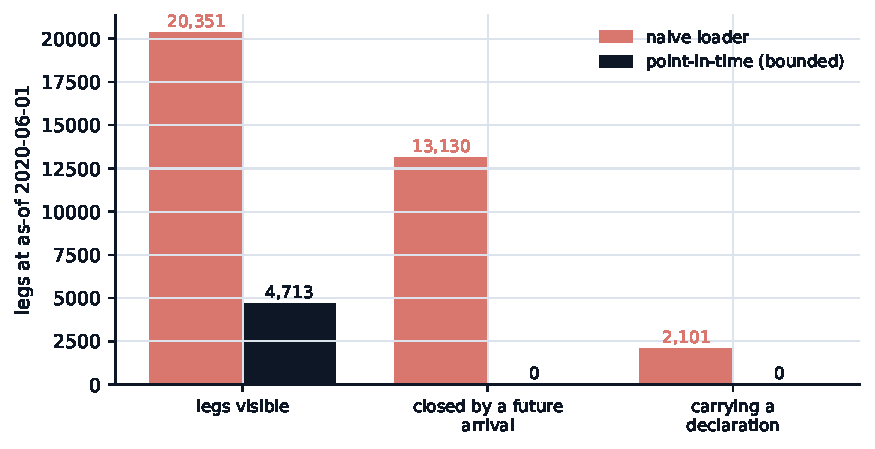
\includegraphics[width=0.95\linewidth]{fig2_leakage}
\caption{Voyage legs visible at an as-of date of 1~June~2020 under the naive loader
and under the point-in-time bound. Recomputed from the event tables when the figure
is generated.}
\label{fig:leakage}
\end{figure}

\subsection{Feature availability changes across vintages}

The same naive loader attached \leakDeclared{} destination declarations to the 2020
legs. Declarations come from a live AIS static-data feed that began in 2026, so no
declaration existed in 2020. This failure differs from the first. A date filter on
the observations is satisfied, because each declaration row carries a timestamp
within the vessel's current voyage, but the table being joined should not exist at
that vintage. The bound therefore reconstructs the declaration from the raw static
messages available at $d$, and at a 2020 as-of date it returns none.

\subsection{What the knowable basis bounds}\label{sec:bounds}

The knowable basis bounds on event time. Event timestamps are back-dated to the fix
at which a transition first qualified, so a departure is dated to the vessel's last
fix inside the berth polygon and not to the later fix that confirmed it had left.
The gap between the two is the feature's own publication lag. We measured it
directly. The first fix after a departure event arrives at a median lag of zero
hours, and more than 24 hours later for 0.3\% of departures on the NOAA feed
($n=1{,}500$) and 1.5\% on the live feed ($n=343$). On the decade panel the lag is
immaterial. On the live feed it is a genuine data limitation: a vessel that drops
out of terrestrial coverage as it leaves the berth is only back-dated once it
reappears, and a satellite feed would remove the gap. This is one of the reasons the
live acquisition system of Section~\ref{sec:live} spends most of its effort on
keeping vessels near terminals in a slot.

A separate log records the knowable value of every signal as it was printed on each
day of live operation, so that the bound can be checked rather than assumed.
Comparing the rebuilt knowable series with those prints on days old enough to have
settled, the check flags \vintagePostDay{} rows whose value moved after a next-day
print. All of them lie in the live tail and are consistent with late-arriving fixes
back-dating departures. A further \vintageSameDay{} rows differ from prints taken
during the day, before that day's fixes had finished arriving. That comparison
measures intraday timing and not leakage; it is reported but not scored. The live
tail lies outside the modelling sample used in Section~\ref{sec:partb}.

\subsection{The modelling grid}

Prices, storage and the tanker signals arrive on different calendars. They are
assembled onto one daily grid by forward-fill under a per-cadence staleness ceiling.
An inner join is never used: \HH{} spot prints on 69\% of calendar days, and an inner
join across the price legs would drop a third of the history without any indication
that it had done so. Each external series is shifted to the date on which it became
public (EIA weekly storage by six days, daily spot by one, AGSI+ by one). The tanker
signals are shifted by zero, because the knowable basis is already point-in-time and
a second shift would double-count. Degree days are not shifted. Their role is to be
partialled out, so the relevant quantity is the weather that occurred and not the
weather that was forecast. Figure~\ref{fig:signals} shows the eight signals that
enter Section~\ref{sec:partb}, on this grid.

\begin{figure*}[tb]
\centering
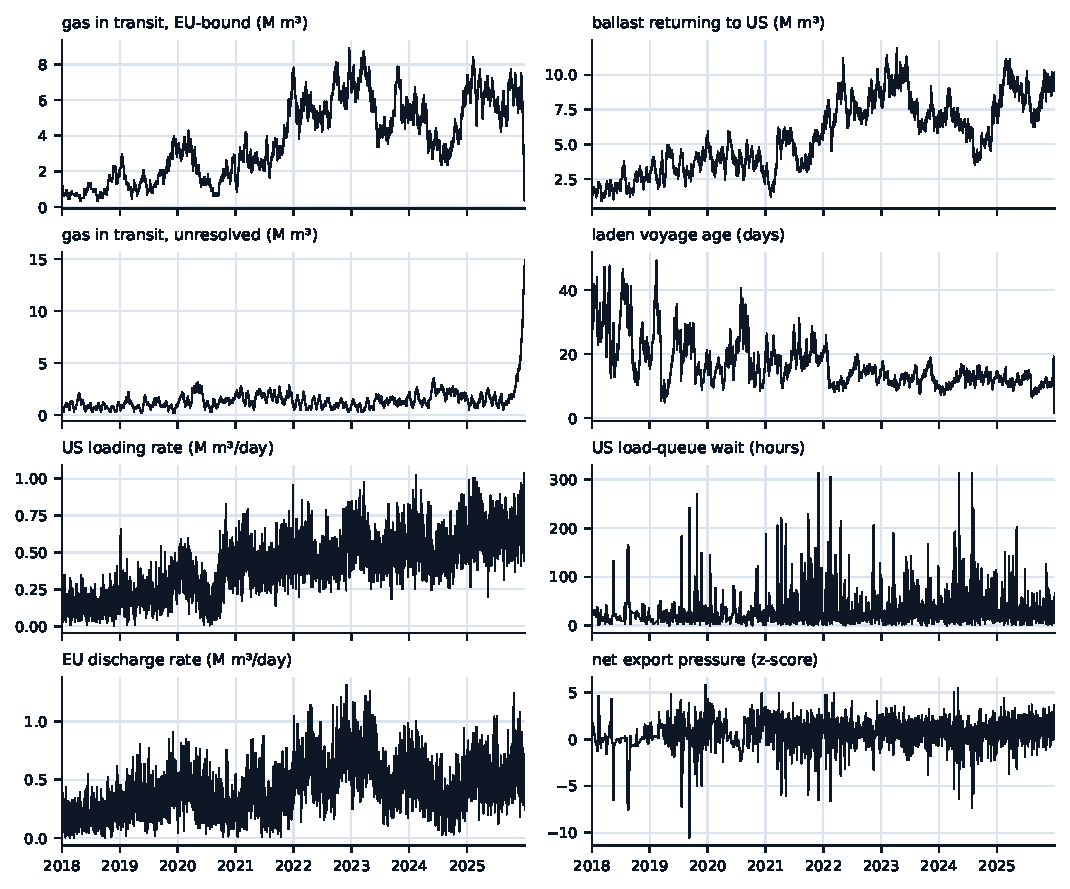
\includegraphics[width=0.95\textwidth]{fig18_signals}
\caption{The eight pre-registered tanker signals, daily on the knowable basis,
2018 to the coverage horizon. The upward drift in the volume signals is the growth
of US export capacity together with the capture gradient of
Figure~\ref{fig:capture}; the spread scan removes both through the persistence
term. The step at the very end of the EU-bound and unresolved in-transit panels is
the coverage seam.}
\label{fig:signals}
\end{figure*}

\subsection{The coverage seam}\label{sec:seam}

The two backfill feeds end on \noaaEnds{} (NOAA) and \gfwEnds{} (GFW). After those
dates the signals are carried by the live feed alone, which contributes
\nLiveEvents{} events against \nBackfillEvents{} from the backfills
(Figure~\ref{fig:coverage}). The EU-bound stock at sea falls from
\stockDecTwentyFive{} to \stockJanTwentySix{} million\,m$^3$ between December~2025
and January~2026, a \coverageDropShare{} drop with no physical cause. This was found
by plotting Figure~\ref{fig:spread} and was not caught by any automated check. The
primary modelling sample is therefore truncated at \noaaEnds. Full-panel results are
reported in Appendix~\ref{app:fullpanel} and change no conclusion.

\begin{figure*}[tb]
\centering
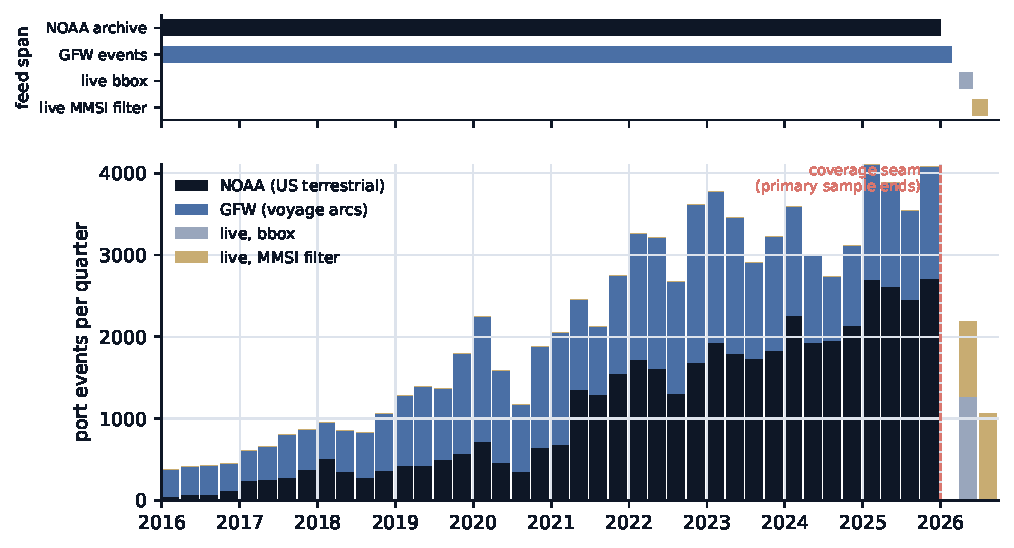
\includegraphics[width=0.95\textwidth]{fig6_coverage}
\caption{Port events per quarter by the feed that produced them, with the span of
each feed above. The NOAA and GFW backfills carry the decade; the live feed, split at
the cutover from a bounding-box subscription to a vessel-identifier filter, carries
only the tail. The dashed line is the coverage seam at which the primary sample ends.}
\label{fig:coverage}
\end{figure*}

\section{Pre-registration protocol}\label{sec:prereg}

The project keeps a dated, append-only decision log. A hypothesis, target, lag, sign
or acceptance bar is committed the day its entry lands, before the corresponding fit;
a later change is a visibly dated superseding entry that names the result which
prompted it. The log is the instrument that turns a null into a finding: without it,
a reader cannot distinguish ``we tested and found nothing'' from ``we kept looking
until nothing crossed a line, and reported the line''. Table~\ref{tab:prereg} lists
the entries that fixed each model below.

\begin{table}[t]
\centering\small
\caption{Pre-registration entries. The commit column is the honest part: see the text.}
\label{tab:prereg}
\begin{tabular}{llp{7.2cm}l}
\toprule
entry & dated & what was fixed before the fit & commit \\
\midrule
  D-001--D-003 & 2026-08-10 & A1 target, kernel, replay protocol & \texttt{4239d13} \\
  D-016 & 2026-08-12 & A2 design lock & \texttt{4239d13} \\
  D-019 & 2026-08-12 & A5 design lock & \texttt{4239d13} \\
  D-022 & 2026-08-12 & A4 design lock & \texttt{4239d13} \\
  D-025 & 2026-08-12 & H1 horizon test pre-specified & \texttt{4239d13} \\
  D-028 & 2026-09-05 & Part B null + FWL: target, controls, HAC lag, signs & \texttt{e483a1b} \\
  D-031 & 2026-09-05 & H2/H3/H4: signs, Bonferroni bar, holdout & \texttt{c489550} \\
\bottomrule
\end{tabular}

\end{table}

Two consequences of the protocol are visible in the results. A pre-registered sign
falsified by the data is reported as falsified (Section~\ref{sec:parta}); and a test
that produced an apparent 87\% improvement over its null was withdrawn, because the
protocol's own comparability condition failed (Section~\ref{sec:parta}). Neither
would have happened without a committed criterion to fail against.

\paragraph{What the log does not establish.} The log is an ordinary text file in the
project's version control, and its git history does not independently prove the
ordering it asserts. The entries for the physical nowcasts (D-001 through D-026) were
committed together, weeks after the work they describe; the two spread
pre-registrations (D-028 and D-031) were each committed in the same change as their
result. The \emph{substance} of the pre-registration --- the signs, bars, horizon and
holdout fixed in each entry's text --- was written before the corresponding run, but
a sceptical reader has only the author's word for it. We state this rather than have
it discovered, and note that a third-party timestamped registry would have cost
nothing. Future entries are committed and pushed before the run they govern.

\section{Physical nowcasts}\label{sec:parta}

Before asking whether the signals predict a price, we ask whether they predict the
physical quantities they measure directly: weekly EU arrivals, weekly US loadings
and terminal outages, at one- and two-week horizons. These targets have high
signal-to-noise ratios and published ground truth, and they establish what the
pipeline can and cannot see before any price enters the analysis. The models are
labelled A1 to A5 in the order they were pre-registered in the project plan (Part~A
of the plan is the physical layer, Part~B the spread); A3, a survival model of
voyage time, was specified but not built, for reasons recorded in the log. Four
models were pre-registered and scored walk-forward against two naive nulls, and
each was designed to address the diagnosed weakness of the previous one.

\paragraph{Targets, nulls and scoring.} Time is a weekly grid of Mondays from
2018. For an as-of date $t$ the forecast windows are $W_k = (t + 7(k-1),\, t + 7k]$
days, and the target is a count of cargoes in the window: the conditional EU
arrival count for A1 (laden legs already at sea at $t$ whose first European zone
entry falls in $W_k$) and the US laden-departure count for A2 and A4. The
\term{persistence} null is the last fully elapsed week's count, and the
\term{climatology} null is the trailing four-week mean; both are computable at $t$.
Models are scored by mean absolute error (MAE) in cargoes, and a model
\term{beats} a null when its MAE is lower. We report each model's excess error over
the climatology null,
\begin{equation}
  \text{excess} = \frac{\mathrm{MAE}_{\text{model}} - \mathrm{MAE}_{\text{clim}}}{\mathrm{MAE}_{\text{clim}}},
  \label{eq:excess}
\end{equation}
so that a positive value is worse than the null. Calibration is scored by the share
of outcomes inside the model's central 80\% interval, which should lie between 70
and 90\%. The pre-registered bar was to beat both nulls on one-week MAE and to land
inside that coverage band. Figure~\ref{fig:loadings} shows the loadings series the
US-side models forecast, with both nulls drawn on it.

\begin{figure*}[tb]
\centering
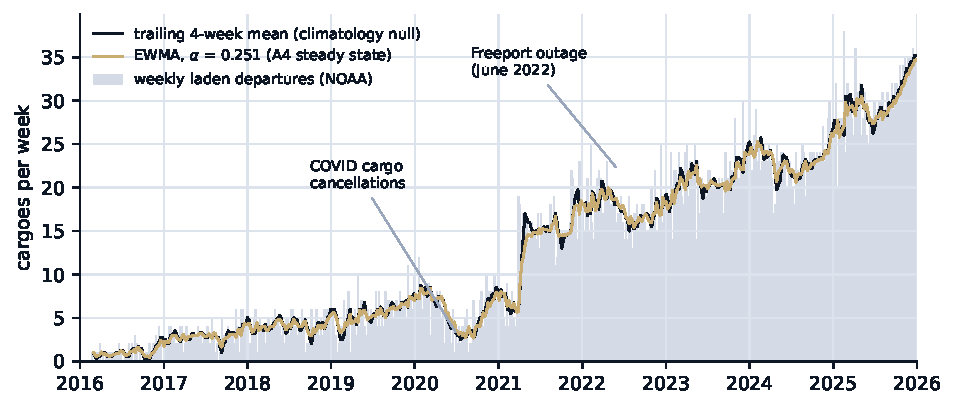
\includegraphics[width=0.95\textwidth]{fig11_loadings}
\caption{Weekly laden departures from US export terminals on the NOAA feed, with
the two objects the nowcasts compete against: the trailing four-week mean (the
climatology null) and the exponentially weighted moving average at the smoothing
constant A4 fitted by maximum likelihood, $\alpha=\aFourAlphaFig$. The series
peaks at \loadingsWeeklyPeak{} cargoes in a week and averages
\loadingsWeeklyMeanTwentyFive{} per week in 2025. The 2020 trough is the COVID
cargo-cancellation wave and the mid-2022 step down is the Freeport outage.}
\label{fig:loadings}
\end{figure*}

\paragraph{A1: duration climatology.} For each open laden leg $i$ of age $a$ at $t$,
the probability that it produces an observed European arrival in $W_k$ is
estimated directly as a count ratio over the matured population of the trailing
year,
\begin{equation}
  p_i(W_k) = \frac{N_{\mathrm{eu}}\!\left(\text{duration} \in (a+u_0,\, a+u_1]\right)}{N(\text{open at age } a)},
  \label{eq:a1}
\end{equation}
where $(u_0, u_1]$ is the window offset. The ratio factorises into an
age-conditional probability that the leg is Europe-bound at all and the duration
distribution of Europe-bound legs, but because both come from one population the
factors telescope into the single ratio above. The weekly count is the
Poisson-binomial sum over open legs, with mean $\sum_i p_i$ and an exact
probability mass function by convolution. A1 has no fitted parameter.

\paragraph{A2: negative-binomial count model.} Weekly US loadings $y$ are modelled
as
\begin{equation}
  \log \lambda = \beta_0 + \sum_j \beta_j x_j, \qquad y \sim \mathrm{NB}(\lambda, k),
  \label{eq:a2}
\end{equation}
with five features fixed in advance together with their expected signs: last
week's count, the trailing four-week mean, the number of vessels in berth, ballast
arrivals in the past week, and the anchorage queue depth. The first two features
are the two nulls, so the scorecard asks whether the three physical features add
anything to the autoregression. Coefficients are refit every week on an expanding
window with a minimum of 104 weeks.

\paragraph{A4: Kalman local level.} The same target is modelled as a latent weekly
rate observed with noise,
\begin{equation}
\begin{aligned}
  x_t &= x_{t-1} + w_t, & w_t &\sim N(0, q), \\
  y_t &= x_t + v_t,     & v_t &\sim N(0, r),
\end{aligned}
\label{eq:a4}
\end{equation}
with $(q, r)$ by exact maximum likelihood, walk-forward. In steady state the
filter's one-step forecast is an exponentially weighted moving average,
$\hat{x}_t = \alpha y_t + (1-\alpha)\hat{x}_{t-1}$, with $\alpha$ set by the ratio
$q/r$ and an effective window of $(2-\alpha)/\alpha$ weeks. A4 therefore asks
whether an optimally tuned moving average beats the fixed four-week one.

\begin{table*}[tb]
\centering\small
\caption{One-week-ahead nowcasts of weekly US loadings (A2, A4) and conditional EU
arrivals (A1), scored walk-forward from 2018 on the NOAA feed. MAE is in cargoes per
week; the excess column is Equation~\eqref{eq:excess}. All three fail the
pre-registered bar of beating both nulls.}
\label{tab:parta}
\begin{tabular}{lrrrrr}
\toprule
model & MAE & persistence & climatology & vs climatology & 80\% cov. \\
\midrule
  A1 arrival-count climatology & 2.314 & 2.217 & 1.814 & +27.5\% & 73.7\% \\
  A2 negative-binomial GLM & 3.961 & 2.551 & 2.152 & +84.0\% & 75.7\% \\
  A4 Kalman local level & 2.104 & 2.694 & 2.088 & +0.7\% & 72.6\% \\
\bottomrule
\end{tabular}

\end{table*}

\begin{figure}[t]
\centering
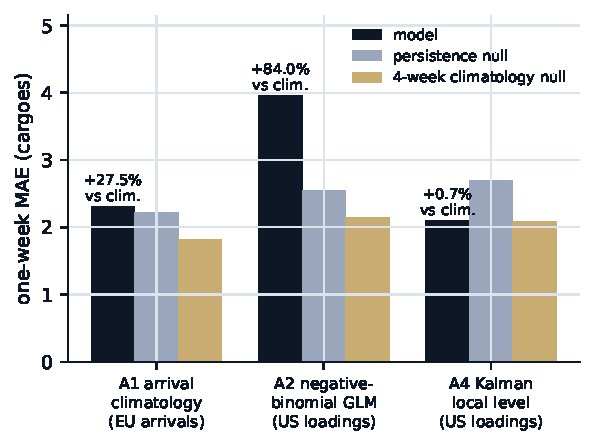
\includegraphics[width=\linewidth]{fig12_parta}
\caption{One-week MAE of each model against its two nulls, from
Table~\ref{tab:parta}. No model beats the four-week climatology; A4 ties it.}
\label{fig:parta}
\end{figure}

\paragraph{Results.} Table~\ref{tab:parta} and Figure~\ref{fig:parta} give the
one-week results. A1 is \aOneSkill{} worse than the climatology null; its estimator
is built from legs at least ninety days old inside a one-year window, so it is
stale, and its errors are the classic lag pattern of under-shooting on the way up
and over-shooting on the way down. A2 is \aTwoSkill{} worse because it
over-extrapolates the trend: the log link on an expanding window places current
features several standard deviations above the training mean and the exponential
converts that distance into multiplicative overshoot. A2 also falsified one of its
pre-registered signs: ballast arrivals entered with coefficient \aTwoBallastCoef{}
against a prior of positive. A4, the Kalman local-level model, is \aFourSkill{}
from the null, which we treat as a tie. The tie carries information. A4 fitted its
smoothing constant by maximum likelihood and chose $\alpha=\aFourAlpha$, an
effective window of \aFourWindow{} weeks. For a series that is a local level plus
noise, the exponentially weighted moving average is the optimal linear predictor
\citep{muth1960}. The fitted model landing next to a four-week simple average
indicates that the optimum was found, and not that four methods happened to tie. On
this target and at this horizon, the naive mean is close to optimal, and a fifth
method would not have changed the conclusion. The sequence is not a monotone
convergence: A2 was the worst of the four, not the middle rung.

\paragraph{A5: outage detection.} A5 tested Bayesian online change-point detection
\citep{adams2007} on each US terminal's daily laden-departure count against
\aFiveOutages{} labelled outages over \aFiveTerminalYears{} terminal-years. The
observation model is Poisson with a Gamma prior on the rate, and the detector
maintains a posterior over the run length $r_t$ (days since the last change) by
\begin{equation}
\begin{aligned}
  P(r_t = r+1) &\propto P(r_{t-1} = r)\, \pi(y_t \mid r)\,(1-H), \\
  P(r_t = 0)   &\propto \textstyle\sum_r P(r_{t-1} = r)\, \pi(y_t \mid r)\, H,
\end{aligned}
\label{eq:bocpd}
\end{equation}
where $\pi(y_t \mid r)$ is the run's negative-binomial posterior predictive and
$H$ the hazard; it alarms when the run-length-averaged rate falls below a fixed
fraction of the pre-change rate. The nulls are two silence rules that read the
time since the last departure: N1 alarms after a fixed 14~days, N2 after five times
the terminal's own baseline inter-departure interval. Table~\ref{tab:parta5} and
Figure~\ref{fig:outage} give the scorecard. BOCPD did not outperform the
rate-relative rule, because daily binning discards the exact timing that a point
process carries: about half of normal days are zero-count at a two-day cadence, so
each zero is weak evidence. N2 detects with a median delay of \aFiveNTwoDelay{}
days at \aFiveNTwoFar{} false alarms per terminal-year, with recall
\aFiveNTwoRecall{} (\aFiveNTwoHits); every miss is a slow-baseline terminal whose
five-times rule exceeds the 21-day detection window. It is a usable but limited
monitor, and it is the baseline rather than the proposed model. Its use should be
stated plainly: a twelve-day median delay is slower than public news of a terminal
outage, so N2 is an automated cross-check on the reconstruction rather than an
alert a trader would act on.

\begin{table*}[tb]
\centering\small
\caption{Outage detection against labelled terminal outages. N2 is the pre-registered
null and the usable artefact; its recall is the relevant number.}
\label{tab:parta5}
\begin{tabular}{lrrr}
\toprule
detector & recall & median delay (d) & false alarms / terminal-yr \\
\midrule
BOCPD (pre-registered) & 12\% (2/16) & 17 & 0.13 \\
N1 absolute silence (14 d) & 88\% (14/16) & 14 & 2.33 \\
N2 rate-relative silence & 38\% (6/16) & 12 & 0.19 \\
\bottomrule
\end{tabular}

\end{table*}

\begin{figure}[t]
\centering
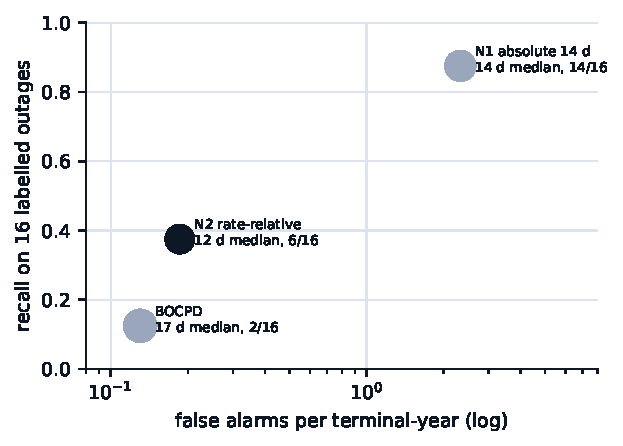
\includegraphics[width=\linewidth]{fig14_outage}
\caption{Recall against false alarms for the three detectors; marker size grows
with median delay. N1's recall is near-tautological, since a labelled outage is by
construction a gap of at least fourteen days, and its false-alarm rate is the real
story.}
\label{fig:outage}
\end{figure}

\paragraph{A withdrawn test.} A natural extension asks whether skill rises with
horizon, since cargo at sea today determines arrivals two to three weeks ahead. This
was pre-specified before any longer-horizon data was examined, with the premise,
also written down, that the nulls would degrade with horizon. The test extends the
A1 window index to $k=1,\dots,4$ and scores each $W_k$ against the same two nulls.
Extending to four weeks produced a \hOneSkillWFour{} improvement over the best null
at week four (Table~\ref{tab:h1}). The improvement is an artefact, and
Figure~\ref{fig:h1} shows why. A1's target is conditional on legs already at sea at
$t$, whereas both nulls are the last elapsed \emph{unconditional} weekly count. The
two coincide at one and two weeks, because no US-to-EU voyage completes in under
seven days, so nothing arrives in the first week that had not already departed.
Past the voyage tail the conditional truth falls toward zero (mean
\hOneTruthWOne{} arrivals in week one and \hOneTruthWFour{} in week four) while the
nulls continue to predict the full weekly rate (\hOnePersistWFour{} MAE). A1 was
forecasting a smaller quantity, not forecasting better; a forecast of zero would
have scored almost as well. The pre-specified premise fails, and the protocol
treats that outcome as grounds to abandon the test. In the comparable region, the
excess moves from \hOneSkillWOne{} to \hOneSkillWTwo{}, which is the predicted
direction but remains below the null. A valid horizon test needs an unconditional
target, which requires composing A1 with a departure-process model such as A2; that
composition is listed as future work.

\begin{table*}[tb]
\centering\small
\caption{A1 extended to four weekly windows. The skill column at W3 and W4 is an
artefact of a conditional target scored against unconditional nulls; the harness no
longer reports it as a result.}
\label{tab:h1}
\begin{tabular}{lrrrrrr}
\toprule
window & mean truth & A1 MAE & persistence & climatology & ``skill'' & 80\% cov. \\
\midrule
  W1 & 5.89 & 2.324 & 2.226 & 1.822 & $-$27.5\% & 73.5\% \\
  W2 & 5.49 & 2.121 & 2.052 & 1.773 & $-$19.6\% & 76.0\% \\
  W3 & 1.98 & 1.170 & 4.146 & 4.058 & +71.2\% & 85.9\% \\
  W4 & 0.75 & 0.691 & 5.247 & 5.208 & +86.7\% & 94.2\% \\
\bottomrule
\end{tabular}

\end{table*}

\begin{figure}[t]
\centering
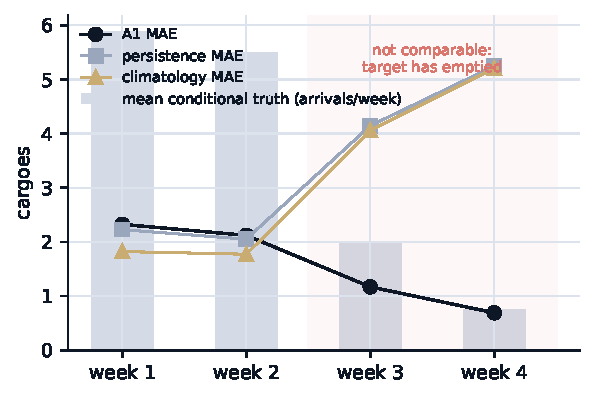
\includegraphics[width=\linewidth]{fig13_h1}
\caption{The withdrawn horizon test. Bars are the mean conditional truth in each
window; lines are the MAE of A1 and of the two nulls. Beyond week two the target
empties while the nulls keep forecasting a full week's arrivals, so the apparent
skill measures the target changing meaning.}
\label{fig:h1}
\end{figure}

\section{The spread}\label{sec:partb}

\subsection{Target, grid and controls}

The target is the spread $\spread = \text{HH}_t - \text{TTF}_t$ in \$/MMBtu, with TTF
converted from EUR/MWh at the day's EUR/USD rate and 3.412\,MWh per MMBtu. It is
sampled weekly on Mondays from 2018, the same grid as the physical nowcasts. The
scored quantity is the $h$-week-ahead change, $\Delta_h = s_{t+7h}-s_t$, for
$h\in\{1,4\}$. The level is too persistent to score usefully, because a model that
predicts the current value performs well on it. The primary sample runs to
\noaaEnds{} (Section~\ref{sec:panel}) and contains \bWeeksCov{} complete weeks.

The control block consists of the spread's non-tanker drivers: heating and cooling
degree days for the US and north-west Europe, US and EU storage, Brent, and a winter
dummy. The price legs that construct the target are excluded as regressors. All
standard errors are Newey--West \citep{neweywest1987} with the lag fixed in advance
at $h+1$ weeks. On a weekly grid with $h=4$, consecutive targets share three weeks,
and an ordinary least-squares standard error is roughly $\sqrt{h}$ too small. Fits
are walk-forward with an expanding window and a 104-week minimum. A training row is
admissible only if its target closed strictly before the test week, with a further
one-week embargo \citep{lopezdeprado2018}.

\subsection{The controls-only null is worse than no change}

Three models form a ladder in which each is the null for the next. M0 predicts no
change. M1 is an AR(1) in the level. M2 adds the controls and is the AR(1)+controls
null that the tanker signals were pre-registered to beat. Table~\ref{tab:ladder}
shows that M2 does not beat M0. Relative to a no-change forecast, M2 scores
\bMTwoSkillHOneCov{} at one week and \bMTwoSkillHFourCov{} at four. It is worse at the
longer horizon and worse in each of 2023, 2024 and 2025 taken individually. This is
the behaviour expected of an efficient and persistent price series: the level already
incorporates the fundamentals, so adding them as regressors introduces estimation
noise. The operative null for the signals is therefore M0, a stricter bar than the
one pre-registered.

\begin{table}[t]
\centering\small
\caption{The model ladder on the primary sample. Skill is the fractional MAE
improvement over M0; a negative value means worse than a no-change forecast.}
\label{tab:ladder}
\begin{tabular}{llrrrrr}
\toprule
$h$ (wk) & model & $n$ & MAE & RMSE & 80\% cov. & skill vs M0 \\
\midrule
  1 & M0 & 272 & 2.034 & 4.465 & 81.6\% & -- \\
  1 & M1 & 272 & 2.061 & 4.571 & 81.6\% & -1.4\% \\
  1 & M2 & 272 & 2.223 & 4.630 & 82.4\% & -9.3\% \\
  4 & M0 & 266 & 3.942 & 7.203 & 72.9\% & -- \\
  4 & M1 & 266 & 4.196 & 7.585 & 70.7\% & -6.4\% \\
  4 & M2 & 266 & 4.660 & 7.437 & 69.5\% & -18.2\% \\
\bottomrule
\end{tabular}

\end{table}

\subsection{No signal survives partialling}

For each of eight pre-registered signals we residualise both the target and the
signal on M2's regressors and regress residual on residual. This is the
Frisch--Waugh--Lovell partial effect \citep{frischwaugh1933,lovell1963}. By the
theorem it equals the signal's coefficient in the full regression, and that equality
serves as the harness's correctness test. Each signal carried a sign fixed in advance
(Appendix~\ref{app:signals}). A result counted only if $|t|>1.96$, the sign matched,
and the sign held in at least two-thirds of individual years. The last condition
guards against 2022 alone driving a pooled fit.

\begin{figure}[t]
\centering
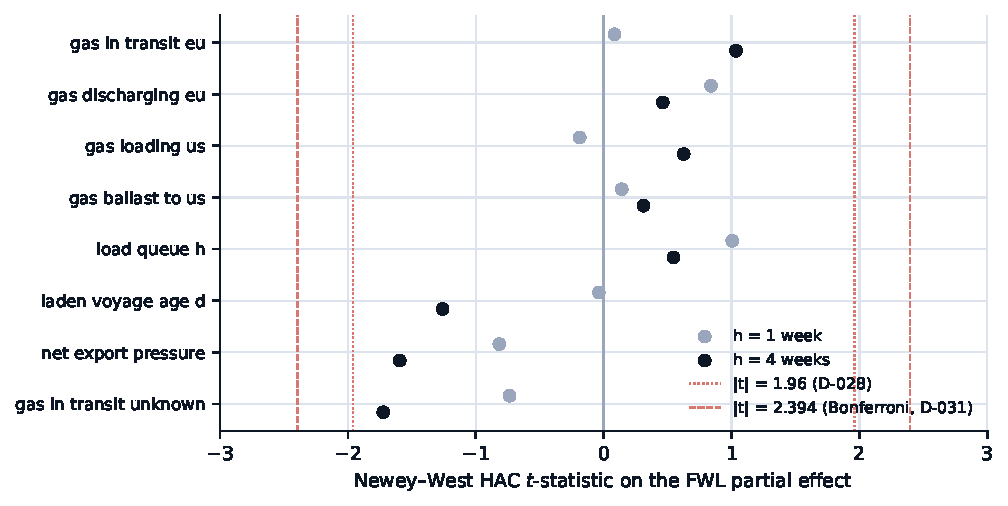
\includegraphics[width=0.9\linewidth]{fig3_fwl_scan}
\caption{Newey--West $t$-statistics on the FWL partial effect of each pre-registered
signal, after controlling for persistence, weather, storage and oil, at one and four
weeks. The dotted and dashed lines mark the two decision bars used in the paper.}
\label{fig:fwl}
\end{figure}

\begin{table}[t]
\centering\small
\caption{FWL partial effects on the primary sample. Year consistency is the share of
individual years whose partial effect has the full-sample sign.}
\label{tab:fwl}
\begin{tabular}{llrrrrr}
\toprule
 & & \multicolumn{2}{c}{$h=1$} & \multicolumn{2}{c}{$h=4$} & \\
\cmidrule(lr){3-4} \cmidrule(lr){5-6}
signal & prior & HAC $t$ & partial $R^2$ & HAC $t$ & partial $R^2$ & year cons. \\
\midrule
  gas in transit, EU-bound & $+$ & +0.18 & 0.000 & +1.40 & 0.009 & 62\% \\
  gas in transit, unresolved & none & -0.03 & 0.000 & +0.24 & 0.000 & 50\% \\
  US loading rate & $+$ & -0.32 & 0.000 & +1.14 & 0.006 & 62\% \\
  EU discharge rate & $+$ & +0.83 & 0.001 & +1.21 & 0.003 & 62\% \\
  ballast returning to US & $+$ & +0.61 & 0.001 & +1.50 & 0.008 & 62\% \\
  laden voyage age & $-$ & +0.02 & 0.000 & -1.14 & 0.004 & 62\% \\
  US load-queue wait & $-$ & +0.78 & 0.001 & +0.07 & 0.000 & 38\% \\
  net export pressure & $+$ & -0.49 & 0.000 & -1.11 & 0.003 & 75\% \\
\bottomrule
\end{tabular}

\end{table}

No signal meets the bar (Figure~\ref{fig:fwl}, Table~\ref{tab:fwl}). The largest
$|t|$ at either horizon is \bMaxTCov, and the largest \pRsq{} is \bMaxRsqCov. The
most direct mechanical hypothesis, that cargo at sea today lands in Europe in two to
three weeks, was tested as the EU-bound stock and gave $t=\bTransitTOneCov$ at one
week and $\bTransitTFourCov$ at four. At four weeks the four flow signals all have
their pre-registered sign, but all lie well inside the noise band. They are
directionally consistent with the mechanism and uniformly insignificant. No sign was
falsified, because no estimate reached significance.

\subsection{Three mechanisms a linear scan could miss}

A one-at-a-time linear scan has three identifiable blind spots. Each was tested with
a derived feature or a sample split, so each costs a single test. The three were
pre-registered together with a Bonferroni bar of $|t|>\bonferroniT$, a primary
horizon of four weeks chosen from the voyage mechanism, and a holdout
(\mechHoldLoCov{} to \mechHoldHiCov, \mechHoldNCov{} weeks) that was not examined
until a hypothesis had passed on the discovery sample (\mechDiscLoCov{} to
\mechDiscHiCov, \mechDiscNCov{} weeks). A pass required the holdout sign to match.

H2 tests the share of cargo bound for Europe in place of the level. Most of the
at-sea stock has no resolved destination, so two collinear levels with offsetting
effects could each appear insignificant while their ratio carries the signal. A
pre-registered gate voids the test if the share is mostly a decade-long trend, which
would indicate improving coverage rather than changing cargo routing. The trend
explains $\Rsq=\mechTrendRsqCov$ and the gate passes. H3 tests an interaction with EU
storage. Additional cargo arriving when storage is 90\% full has little effect,
while the same cargo at 30\% is highly price-relevant, and a linear fit averages the
two states. H4 tests a tightness split, the simplest form of a regime model. The
scan is re-run within weeks in which EU storage is below its seasonal norm (with the
norm fitted on the discovery sample only), and the prediction is that the effect is
positive in those weeks and larger than in the remaining weeks.

\begin{table}[t]
\centering\footnotesize
\caption{The three pre-registered mechanism tests on the discovery sample at $h=4$
with Bonferroni bar $|t|>\bonferroniT$. None is significant. H3 has the wrong sign,
and H4's tight-regime effect is smaller than its loose-regime effect.}
\label{tab:mechanisms}
\begin{tabular}{llrrrrr}
\toprule
hypothesis & prior & $\hat\beta$ (discovery) & HAC $t$ & year cons. & partial $R^2$ & $\hat\beta$ (holdout) \\
\midrule
  H2: EU share of at-sea stock & $+$ & $-2.64 \times 10^{0}$ & -0.89 & 71\% & 0.003 & $-2.51 \times 10^{0}$ \\
  H3: transit $\times$ EU storage & $-$ & $4.78 \times 10^{-9}$ & +0.46 & 71\% & 0.001 & $-1.49 \times 10^{-9}$ \\
  H4: transit, tight regime & $+$ & $-1.13 \times 10^{-7}$ & -0.17 & 100\% & 0.000 & $2.71 \times 10^{-7}$ \\
  H4: transit, loose regime & $+$ & $-2.25 \times 10^{-7}$ & -1.00 & 100\% & 0.009 & -- \\
\bottomrule
\end{tabular}

\end{table}

All three fail (Table~\ref{tab:mechanisms}), and none approaches the bar. The
largest $|t|$ among the primary tests is \mechMaxTCov. Each failure argues against a
further attempt. The H2 estimate is stable and negative on both discovery
(\mechHTwoBetaCov) and holdout (\mechHTwoHoldCov), which is the wrong sign, and it
never approaches significance. H3 is positive ($t=\mechHThreeTCov$) against a prior
of negative, so neither the magnitude nor the direction of the storage interaction
is present. H4's tight-regime effect is negative ($t=\mechHFourTightTCov$) and
smaller in magnitude than the loose-regime effect, which reverses both predictions.
On this evidence, cargo arrivals do not have a measurable effect in either storage
state.

The linear null of the previous subsection has thus been tested against the three
specific ways in which it could have been wrong, using pre-registered signs, a
corrected bar and an untouched holdout, and it stands.

\section{What the design could have found}\label{sec:power}

A null result is informative only in proportion to the smallest effect it could
have detected. For a partial effect estimated on $n$ observations,
$t^2 \approx n\,R^2/(1-R^2)$, so at a fixed bar $t^\ast$ the smallest detectable
\pRsq{} is
\begin{equation}
  R^2_{\min} = \frac{t^{\ast 2}}{n + t^{\ast 2}},
  \label{eq:power}
\end{equation}
which falls as $1/n$. With \powerN{} discovery weeks and the Bonferroni bar of
$|t|>\bonferroniT$, the floor is \powerFloor{} of residual variance
(Figure~\ref{fig:power}). The largest \pRsq{} observed anywhere in the paper, across
eight signals, two horizons, three mechanisms and two samples, is \bMaxRsqCov.

\begin{figure}[t]
\centering
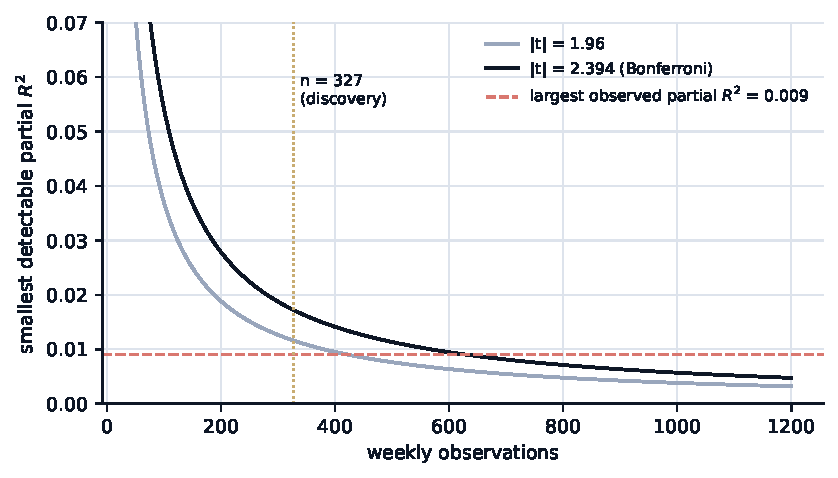
\includegraphics[width=\linewidth]{fig4_power}
\caption{Smallest detectable \pRsq{}, Equation~\eqref{eq:power}, as a function of
sample size at the two bars used in the paper, with the largest observed \pRsq{} and
the discovery sample size marked. Halving the floor needs twice the sample, which
at a weekly grid means another six years of coverage-consistent data.}
\label{fig:power}
\end{figure}

The scope of the result follows from this. It excludes effects large enough to be
traded and is silent on smaller ones. A signal explaining a third of a percent of
residual variance would be physically real and commercially useless, and this design
could not distinguish it from zero. Two facts about scale make the null less
surprising than the intuition that motivated the study. The EU-bound stock of gas at
sea averages \stockMeanMm{} million\,m$^3$ of LNG, which is about
\stockMeanBcm{}\,bcm of gas or \stockDaysDemand{} days of EU demand at roughly
\euDemandBcm{}\,bcm per year. A one-standard-deviation change in that stock is
\stockSdDaysDemand{} days of demand. The weekly spread has a standard deviation of
\$\spreadWeeklySd{} per MMBtu. The question was therefore whether about a day and a
half of marginal supply moves a price that responds to revisions in the weather
forecast.

\paragraph{Distinguishing a physically real signal from a tradeable one.} The
distinction is worth keeping because it is where the interesting work now lies. A
signal is physically real if it predicts the quantity it measures: Part~A is that
test, and the at-sea stock does predict European arrivals, with a lead equal to the
voyage time, because that is arithmetic. A signal is tradeable if its effect on the
price survives the controls at a size above the floor of
Equation~\eqref{eq:power}. The route to the first question is more physical
targets scored against published totals; the route to the second is a lower floor,
which means a longer coverage-consistent sample or a less attenuated regressor, not
a different model.

% PROPOSAL: the author rewrites this section.
\section{Discussion}\label{sec:discussion}

The null is the outcome an efficient market predicts, and it is important to be
precise about which question was asked. LNG cargo tracking is a commercial industry.
Several vendors sell satellite-augmented AIS with proprietary destination inference
to gas trading desks in real time. The signals in this paper are built from public
terrestrial AIS and a free voyage archive, which is a coarser version of what the
marginal trader already has. The test was therefore not whether the physical signal
is informative, but whether public physical data is mispriced in a liquid benchmark
at one- to four-week horizons. A negative answer to that question is close to what
one would expect in advance. What the paper adds is evidence that the negative
result is not an artefact of a defective pipeline, an unlucky specification, or a
search that stopped at the first $t>2$. The pipeline is validated against a
published total, the specification was fixed before the fit, and the search was
corrected for multiplicity and held out.

Three results stand independently of the null. First, the physical nowcasts
converge on the naive mean from above, and for the one-week loadings target this
follows from theory rather than from the particular models tried. The argument
applies to any slow industrial flow series and should temper the expectation that a
richer model will beat a moving average on one. Second, the two construction hazards
of Section~\ref{sec:panel} apply to voyage-derived features in general, and they are
easy to miss even when dates appear to have been handled correctly. The vintage log
that detects them is inexpensive to maintain and, to our knowledge, rarely kept.
Third, the outage rule of Section~\ref{sec:parta} is a usable monitor with a stated
recall.

Several changes could alter the answer. A private information advantage, such as
satellite coverage of the open ocean or a destination model that resolves the
three-quarters of the stock this pipeline cannot, would change the question rather
than the answer and would make the study a test of the vendor's product. Within
public data, the remaining untested approaches are joint rather than marginal fits
(spike-and-slab or partial least squares over the collinear block), a fitted regime
model in place of an observable split, distributed lags of the signals, and the
twenty-six signal keys the panel does not use. Each has a weaker prior than the three
mechanisms already tested, and each faces a larger multiplicity problem against a
residual that has never exceeded \bMaxRsqCov{} of variance. Any of them should be
accompanied by its own pre-registration, its own multiplicity correction, and the
untouched-holdout standard used here.

% PROPOSAL: the author rewrites this section.
\section{Limitations}\label{sec:limitations}

\paragraph{No European anchorage history.} The GFW feed carries port visits but no
anchorage events, so European queue and absorption signals exist only from the 2026
live feed. Four of the five composite signals originally pre-registered as features
for Section~\ref{sec:partb} turned out to have between 9 and 46 daily observations
and were excluded by a documented amendment before any spread fit. The at-sea and
US-side mechanism was tested on the decade; the EU-congestion mechanism could not
be tested.

\paragraph{Destination resolution.} Between 75\% and 83\% of the at-sea stock has no
resolved destination. The EU-bound series is a minority observed slice whose
definition depends on coverage. The unresolved band is carried as its own feature,
and the ratio of the two was tested as H2. Attenuation from this measurement error
biases coefficients toward zero and cannot be excluded as a contributing factor.

\paragraph{The capture gradient.} NOAA-only capture of US export cargoes is
\captureTwentyTwenty{} in 2020 and \captureTwentyEighteen{} in 2018
(Table~\ref{tab:capture}). Early-year levels of every US signal are biased low. The
walk-forward designs operate on within-window changes and the FWL scan on residuals,
but a level-dependent non-linearity in the early years would be misread.

\paragraph{The coverage seam.} The backfill feeds end on \noaaEnds{} and \gfwEnds.
The full-panel results in Appendix~\ref{app:fullpanel} include the thin live tail.
In that sample 24\% of the holdout weeks lie after the seam, and one full-panel
finding, a change of sign in the H2 holdout coefficient, did not survive truncation
and is not claimed. The primary sample is truncated at the seam.

\paragraph{Regime pooling.} Signals are read from the pooled regime tag, which is
the only tag spanning the decade. A small residual over-count where NOAA and GFW both
observe the same US departure is documented in the project's signal catalogue. A
robustness run on the NOAA tag alone for the US-side signals was not performed.

\paragraph{The pre-registration trail.} As Section~\ref{sec:prereg} states, the git
history does not independently establish that the log entries preceded the fits they
govern.

\paragraph{Sample size and a dominant regime.} The scored spread sample is
\bWeeksCov{} weeks, heavily autocorrelated, and 2022 alone spans a range larger than
the remainder of the decade combined. The year-consistency condition and the holdout
are the defences against this; a longer sample without a coverage seam would be
preferable to either.

\paragraph{Vintage residual.} \vintagePostDay{} rows in the live tail changed after a
next-day print (Section~\ref{sec:panel}). They lie outside the modelling sample, but
they show that the knowable bound is exact on event time and only approximately
exact on observation time in a thin-coverage regime.


\bibliographystyle{plainnat}
\bibliography{refs}

\appendix
\section{Signal definitions and pre-registered signs}\label{app:signals}

The eight tanker signals used in Section~\ref{sec:partb}, the aggregation applied
when collapsing per-terminal or per-zone bands to one daily series, and the sign
committed before any fit. The sign convention: the spread $\text{HH}-\text{TTF}$ is
negative in nearly every period, so ``the spread narrows'' means it rises toward
zero --- a positive change.

\begin{center}\small
\begin{tabular}{p{3.4cm}p{1.6cm}p{7.4cm}c}
\toprule
signal & aggregation & mechanism & prior \\
\midrule
gas in transit, EU-bound & sum over EU zones & more cargo landing in Europe soon $\Rightarrow$ TTF falls & $+$ \\
gas in transit, unresolved & sum & destination unknown; no directional prior & none \\
US loading rate & sum over US berths & gas leaves the US balance (HH firms) and reaches Europe (TTF falls) & $+$ \\
EU discharge rate & sum over EU berths & Europe absorbing gas now $\Rightarrow$ TTF falls & $+$ \\
ballast returning to US & sum & tonnage returning to load $\Rightarrow$ future exports up & $+$ \\
laden voyage age & $n$-weighted mean & cargo floating rather than landing $\Rightarrow$ Europe stays tight & $-$ \\
US load-queue wait & $n$-weighted mean & US cannot export $\Rightarrow$ HH softens, Europe starved & $-$ \\
net export pressure & $n$-weighted mean & $z$(loadings) $-$ $z$(load queue); both legs point the same way & $+$ \\
\bottomrule
\end{tabular}
\end{center}

Volumes are in m$^3$ of LNG; loading and discharge rates are amortised m$^3$ per day
across berth hours so that a closed visit integrates to one cargo; ages and waits are
in days and hours respectively. The project's signal catalogue documents the
remaining twenty-six keys, the two bases, and the confidence columns (dispersion,
open fraction, estimated fraction) that accompany every value.

\paragraph{A recorded inconsistency.} The catalogue's own text gave net export
pressure two incompatible signs in two places. The positive sign was adopted on the
economics above and recorded as a prior; the data returned a negative point estimate
at both horizons, at $|t|\le1.6$, which neither confirms nor falsifies it.

\section{Full-panel results}\label{app:fullpanel}

The primary sample is truncated at the backfill horizon (\noaaEnds). The same scans
run to the data maximum (\bWeeksFull{} weeks) are reported here for completeness.
They were the runs first recorded in the decision log, and they change no
conclusion.

\begin{table}[h]
\centering\small
\caption{Model ladder, full panel.}
\begin{tabular}{llrrrrr}
\toprule
$h$ (wk) & model & $n$ & MAE & RMSE & 80\% cov. & skill vs M0 \\
\midrule
  1 & M0 & 288 & 1.997 & 4.371 & 82.3\% & -- \\
  1 & M1 & 288 & 2.023 & 4.473 & 82.3\% & $-$1.3\% \\
  1 & M2 & 288 & 2.205 & 4.542 & 83.0\% & $-$10.4\% \\
  4 & M0 & 282 & 3.947 & 7.090 & 73.8\% & -- \\
  4 & M1 & 282 & 4.168 & 7.444 & 72.0\% & $-$5.6\% \\
  4 & M2 & 282 & 4.705 & 7.378 & 69.1\% & $-$19.2\% \\
\bottomrule
\end{tabular}

\end{table}

\begin{table}[h]
\centering\small
\caption{FWL partial effects, full panel. The largest $|t|$ here (\bMaxTFull)
belongs to the unresolved-destination band and falls to $+0.24$ on the primary
sample. It was produced by the contaminated tail.}
\begin{tabular}{llrrrrr}
\toprule
 & & \multicolumn{2}{c}{$h=1$} & \multicolumn{2}{c}{$h=4$} & \\
\cmidrule(lr){3-4} \cmidrule(lr){5-6}
signal & prior & HAC $t$ & partial $R^2$ & HAC $t$ & partial $R^2$ & year cons. \\
\midrule
  gas in transit, EU-bound & $+$ & +0.08 & 0.000 & +1.03 & 0.004 & 75\% \\
  gas in transit, unresolved & none & -0.74 & 0.001 & -1.72 & 0.009 & 62\% \\
  US loading rate & $+$ & -0.19 & 0.000 & +0.63 & 0.001 & 62\% \\
  EU discharge rate & $+$ & +0.84 & 0.001 & +0.46 & 0.000 & 62\% \\
  ballast returning to US & $+$ & +0.14 & 0.000 & +0.31 & 0.000 & 62\% \\
  laden voyage age & $-$ & -0.04 & 0.000 & -1.26 & 0.005 & 62\% \\
  US load-queue wait & $-$ & +1.01 & 0.001 & +0.55 & 0.001 & 38\% \\
  net export pressure & $+$ & -0.82 & 0.001 & -1.60 & 0.009 & 75\% \\
\bottomrule
\end{tabular}

\end{table}

\begin{table}[h]
\centering\footnotesize
\caption{Mechanism tests, full panel. The holdout coefficient for H2 changes sign
relative to the primary sample. In this sample 24\% of the holdout weeks lie after the
coverage seam, and the change of sign is not claimed as a finding.}
\input{tables/mechanismsfull}
\end{table}

\begin{figure}[h]
\centering
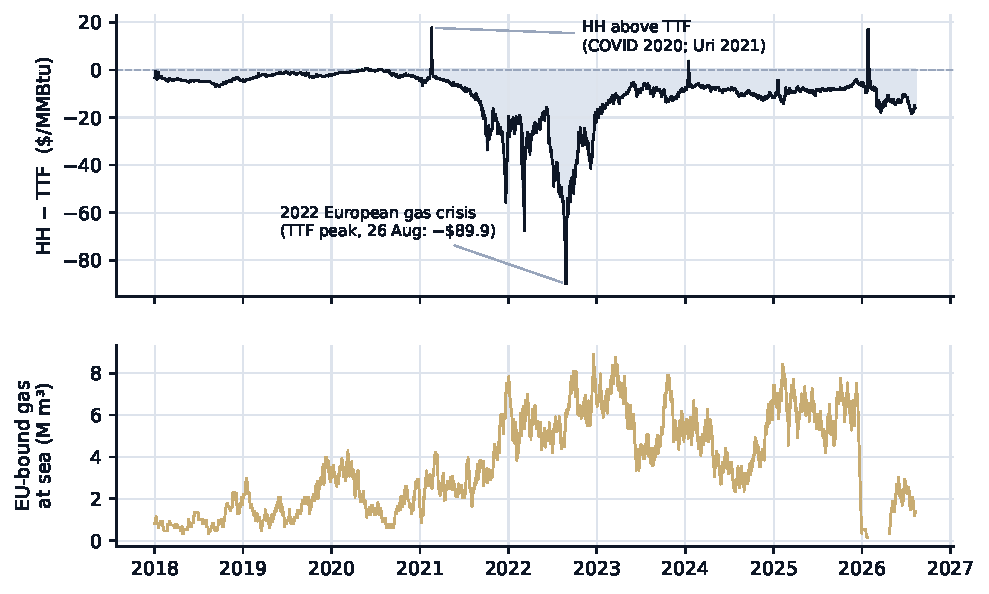
\includegraphics[width=\linewidth]{fig1_spread_and_stock_fullpanel}
\caption{Figure~\ref{fig:spread} extended to the data maximum. The
\coverageDropShare{} step in the at-sea stock at the start of 2026 is the coverage
seam and not a physical event.}
\end{figure}

\begin{figure}[h]
\centering
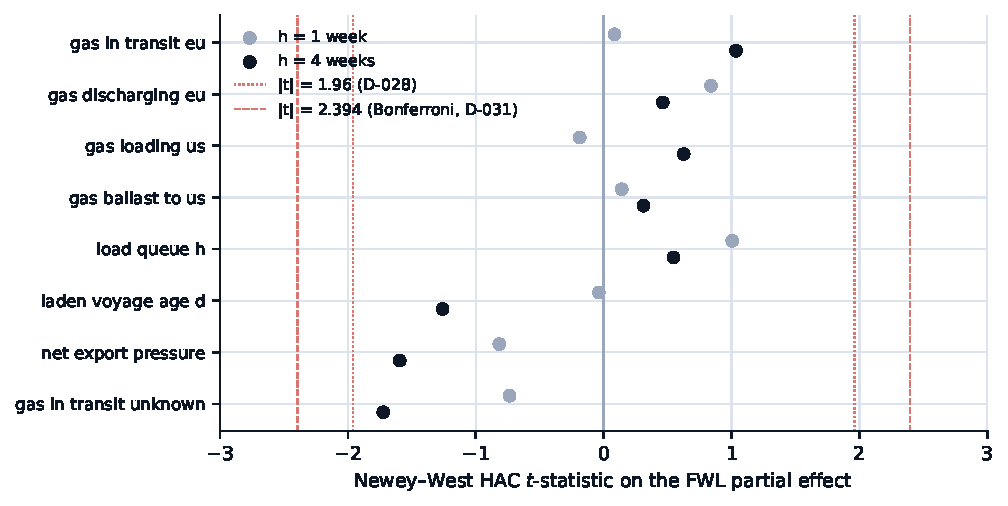
\includegraphics[width=0.9\linewidth]{fig3_fwl_scan_fullpanel}
\caption{Figure~\ref{fig:fwl} on the full panel.}
\end{figure}

\input{sections/appendix_c_repro_ai}

\end{document}
